\documentclass[12pt,a4paper]{report}
\usepackage[utf8]{inputenc}
\usepackage{titlesec}
\usepackage{graphicx}
\usepackage[utf8]{inputenc}
\usepackage[dvipsnames]{xcolor}
\usepackage{color}
\usepackage{imakeidx}
\usepackage[T1]{fontenc}
\usepackage{listings}
\usepackage{fancybox, calc}
\usepackage{hyperref}
\usepackage{amssymb}
\usepackage{keystroke}
\usepackage{tikz}
\usepackage{geometry}
\geometry{
 a4paper,
 total={170mm,257mm},
 left=20mm,
 top=20mm,
 }


\newtheorem{definition}{Definition}

\makeindex
\titleformat{\chapter}[hang]{\normalfont\huge\bfseries}{\chaptertitlename\ \thechapter:}{1em}{}

% Definició dels colors ---------------------------------------------
\definecolor{codegreen}{rgb}{0,0.6,0}
\definecolor{codegray}{rgb}{0.5,0.5,0.5}
\definecolor{codepurple}{rgb}{0.58,0,0.82}
\definecolor{backcolour}{rgb}{0.95,0.95,0.92}

% Definició de l'estil del codi
\lstdefinestyle{mystyle}{
    backgroundcolor=\color{backcolour},
    commentstyle=\color{codegreen},
    keywordstyle=\color{magenta},
    numberstyle=\tiny\color{codegray},
    stringstyle=\color{codepurple},
    basicstyle=\footnotesize,
    breakatwhitespace=false,
    breaklines=true,
    captionpos=b,
    keepspaces=true,
    numbers=left,
    numbersep=5pt,
    showspaces=false,
    showstringspaces=false,
    showtabs=false,
    tabsize=2
}
\lstset{
style=mystyle,
columns=flexible,
breaklines=true,
inputencoding=utf8}


\usepackage{xcolor}
\hypersetup{
    colorlinks,
    linkcolor={red!50!black},
    citecolor={blue!50!black},
    urlcolor={blue!80!black}
}

% VARIABLES
\def \w{$\omega$}
\def \dfa{$DaffyDuck_{DFA} $}
\def \alphabetDFA{$\Sigma$*\dfa}
\def \alphabetPDA{$\Sigma$*\pda}
\def \nfa{$DaffyDuck_{NFA} $}
\def \mfa{$DaffyDuck_{MDFA} $}
\def \wdfa{$\omega_{DFA} $}
\def \wpda{$\omega_{PDA} $}
\def \re{$DaffyDuck_{RE} $}
\def \rg{$DaffyDuck_{rg} $}
\def \cfg{$CFG$}
\def \pdaCFG{$PorkyPigCFG{PDA} $}
\def \pda{$PorkyPig_{PDA} $}
\def \tm{$BugsBunny_{TM} $}
\def \tmz{$BugsBunny_{TM0} $}
\def \tmu{$BugsBunny_{TM1} $}
\def \tml3{$BugsBunny_{TML3} $}
\def \context{$\Phi$}
\def \contextDFA{$\Phi_{DFA}$}
\def \contextPDA{$\Phi_{PDA}$}
\def \contextTM{$\Phi_{TM}$}
\def \pre{$\Upsilon$}
\def \preDFA{$\Upsilon_{DFA}$}
\def \prePDA{$\Upsilon_{PDA}$}
\def \preTM{$\Upsilon_{TM}$}
\def \post{$\Psi$}
\def \postDFA{$\Psi_{DFA}$}
\def \postPDA{$\Psi_{PDA}$}
\def \postTM{$\Psi_{TM}$}
\def \llesca{$\gamma$}
\def \ld{$L^{2}$}

\begin{document}

% Títol de la pràctica -----------------------------------------------
\begin{titlepage}
	\centering
	\includegraphics[width=0.55\textwidth]{udg_logo.png}\par\vspace{1cm}
	{\scshape\LARGE Universitat de girona \par}
	\vspace{1cm}
	{\scshape\Large Pràctica final\par}
	\vspace{1.5cm}
	{\huge\bfseries Fonaments de la computació\par}
	\vspace{2cm}
	{\Large\itshape Francesc Xavier Bullich Parra\par}
	{\Large\itshape Gil Gassó Rovira\par}
	{\Large\itshape Marc Sànchez Pifarré\par}

	\vfill
	Tutor de la pràctica\par
	Jaume Rigau

	\vfill

% Bottom of the page
	{\large \today\par}
\end{titlepage}

% Índex -----------------------------------------------
\tableofcontents
\clearpage


\chapter{Introducció}
\setcounter{chapter}{1}

\section{Definicions}

Es defineixen una sèrie de noms que seran utilitzats al llarg de la pràctica per ajudar a la simplificació i l'enteniment d'aquesta.

\begin{itemize}
\item Definim \dfa{} com l’autòmat finit determinista capaç de reconèixer el llenguatge L(\dfa{}).
\item Definim L (\dfa{}) com el conjunt infinit de mots \w{} que accepta \dfa{}
\item Definim \wdfa{} com un mot tal que \wdfa{} $\in$ L(\dfa{})
\item Definim \alphabetDFA{} com el conjunt de símbols amb el que es construeix el llenguatge L(\dfa{})
\item Definim context \context{} com l’escenari ideal en el que l’autòmat a dissenyar es comportarà de manera correcta, \context{} = < \pre{}, \post{} >
\item Definim \pre{} com la precondició que s'ha de complir a l'utilitzar els nostres autòmats.
\item Definim \post{} com la postcondició de l'autòmat.
\item Definim \pda{} com l'autòmat de Pila capaç de reconèixer el llenguatge L(\pda{}).
\item Definim L(\pda{}) com el conjunt finit de mots $\sigma$ que accepta \pda{}.
\item Definim \wpda{} com un mot del llenguatge L(\pda{}).
\item Definim \alphabetPDA{} com el conjunt de símbols amb el que es construeix el llenguatge L(\pda).

\end{itemize}

\chapter{autòmat Finit}

\section{Definició del context}

Sigui \contextDFA{} l'espai de funcionament lògic del nostre autòmat com l'espai estipulat a la Secció 3. Patrons[2]. Per tant acabem d'adquirir totes les definicions assumides a l'enunciat del problema, veure [2].

\textbf{Fem les següents afirmacions sobre \preDFA{} :}
\begin{itemize}
\item \wdfa{} $\in$ $P_0$ $\wedge$ $P_0$ $\in$ $P$
\item \llesca{} com a llesca continguda dins d'un $P$ on \llesca{} $\in$ \wdfa $\vee$ \llesca{} = $\epsilon$
\end{itemize}

\textbf{Fem les següents afirmacions sobre \postDFA{} :}
\begin{itemize}
\item retorna True quan \dfa{} Accepta \wdfa{} $\leftrightarrow$ $\exists$ \llesca{} $\in$ $P$ que compleix PIP.
\item retorna False quan $\nexists$ \llesca{} $\in$ $P$ que compleix PIP.
\end{itemize}
on : PIP és la propietat dels patrons implícits parcials definida a [2] apartat 3.3.1.

\section{Dissenyant el nostre autòmat finit}

Primerament cal observar possibles propietats del problema que ens puguin servir per a la construcció de l’autòmat.

\begin{itemize}
\item Definim 4+ com la seqüència de símbols ‘++++’ d’un mot \wdfa{} comprés dins del llenguatge L(\dfa{}).
\end{itemize}

\textbf{Realitzem les següents observacions:}

\begin{enumerate}
\item Abans i després de la seqüència 4+ hi pot haver qualsevol símbol 0 o més vegades comprés dins de \alphabetDFA{}.
\item Aïllada és la seqüència de símbols ‘-+-’ dins de \wdfa{}
\item Entre dues seqüències 4+ hi trobem 3 aïllades.
\item 2 aïllades poden compartir el símbol inicial o el símbol final o ambdós.
\item S’accepta ‘-+-+-’ com a dues cèl·lules aïllades on -+ comparteix - amb +-.
\item S’accepta ‘-+-+-+-’ coma  tres cèl·lules aïllades on -+ comparteix- amb +-+- i -+-+ comparteix - amb +-.
\item Entre 2 aïllades hi pot aparèixer qualsevol combinació de símbols pertanyent a \alphabetDFA{}.
\item El símbol \Return ens fa tornar a començar a cercar el PIP (RESET).
\end{enumerate}


Dissenyarem doncs l’autòmat per construcció tenint en compte les anteriors propietats. En la construcció del nostre autòmat reduïm el problema al tractament d’un subconjunt dels símbols de l’alfabet, concretament es construeix a partir del subconjunt {+,-}, ja que detectem que el símbol \Return actua com a RESET. La funció del RESET en \dfa{} és exemplificada al capítol 1 del llibre [1], concretament als exemples 1.15 i 1.17.

Incorporarem el RESET al nostre disseny a l’últim pas de la construcció.

\textbf{Fem les següents definicions en l’escenari sense RESET :}

\begin{itemize}
\item Definim pa com la seqüència ‘-+’
\item Definim fa com la seqüència ‘+-’
\item Definim l’operació CONCATENACIÓ amb el símbol |
\item Definim 3aïllades com :
\begin{itemize}
\item ({+-}* | pa | (-{+-}*)* | pa | (-{+-}*)* | pa | - | {+-}*) $\vee$ ({+-}* | - | fa | (-{+-}*)* | fa | (-{+-}*)* | fa | {+-}*)
\end{itemize}
\end{itemize}

Per tant podem concebre que en un entorn on no hi ha RESET es cerca si el mot conté la següent seqüència de símbols :

\begin{center}
{+-}* | 4+ | 3aïllades | 4+ | {+-}*
\end{center}

\subsection{Construïm l’autòmat sense RESET}

Veiem que els estats de l'autòmat van avançant a mesura que es van trobant el patró. Hi distingim cicles que ens interessen per controlar els casos que on per exemple hi pot haver qualsevol cosa entre cel·les actives o entre cel·les actives i principi o final del patró.

\begin{center}
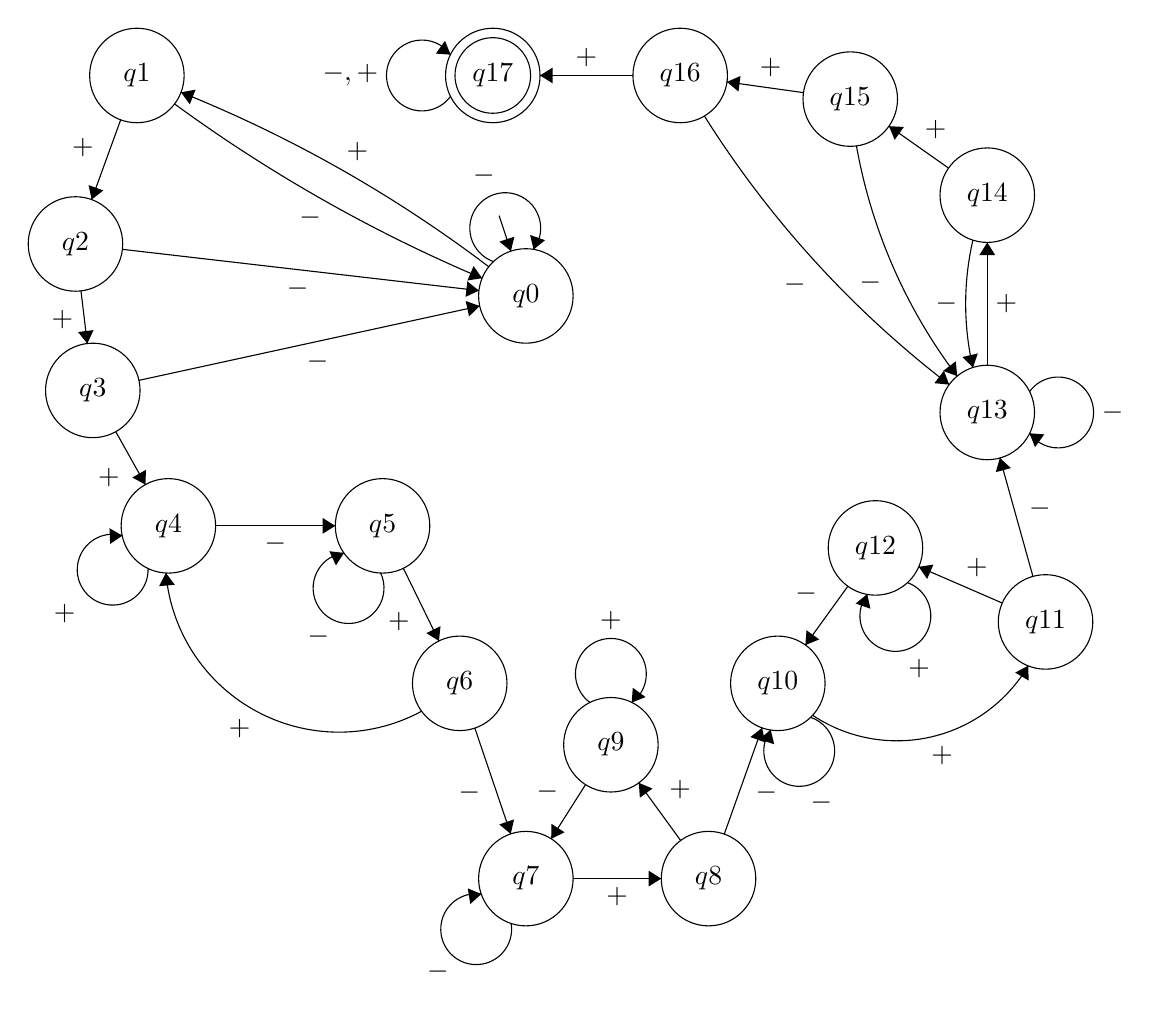
\begin{tikzpicture}[scale=0.2]
\tikzstyle{every node}+=[inner sep=0pt]
\draw [black] (34.2,-17.4) circle (3);
\draw (34.2,-17.4) node {$q0$};
\draw [black] (9.5,-3.4) circle (3);
\draw (9.5,-3.4) node {$q1$};
\draw [black] (5.6,-14.1) circle (3);
\draw (5.6,-14.1) node {$q2$};
\draw [black] (6.7,-23.4) circle (3);
\draw (6.7,-23.4) node {$q3$};
\draw [black] (11.5,-32) circle (3);
\draw (11.5,-32) node {$q4$};
\draw [black] (25.1,-32) circle (3);
\draw (25.1,-32) node {$q5$};
\draw [black] (30,-42) circle (3);
\draw (30,-42) node {$q6$};
\draw [black] (34.2,-54.4) circle (3);
\draw (34.2,-54.4) node {$q7$};
\draw [black] (45.8,-54.4) circle (3);
\draw (45.8,-54.4) node {$q8$};
\draw [black] (39.6,-45.9) circle (3);
\draw (39.6,-45.9) node {$q9$};
\draw [black] (50.2,-42) circle (3);
\draw (50.2,-42) node {$q10$};
\draw [black] (67.2,-38.1) circle (3);
\draw (67.2,-38.1) node {$q11$};
\draw [black] (56.4,-33.4) circle (3);
\draw (56.4,-33.4) node {$q12$};
\draw [black] (63.5,-24.8) circle (3);
\draw (63.5,-24.8) node {$q13$};
\draw [black] (63.5,-11) circle (3);
\draw (63.5,-11) node {$q14$};
\draw [black] (54.8,-4.9) circle (3);
\draw (54.8,-4.9) node {$q15$};
\draw [black] (44,-3.4) circle (3);
\draw (44,-3.4) node {$q16$};
\draw [black] (32.1,-3.4) circle (3);
\draw (32.1,-3.4) node {$q17$};
\draw [black] (32.1,-3.4) circle (2.4);
\draw [black] (12.303,-4.469) arc (68.10472:52.80601:84.368);
\fill [black] (12.3,-4.47) -- (12.86,-5.23) -- (13.23,-4.3);
\draw (23.5,-8.85) node [above] {$+$};
\draw [black] (31.419,-16.275) arc (-112.91179:-126.17748:97.153);
\fill [black] (31.42,-16.27) -- (30.88,-15.5) -- (30.49,-16.42);
\draw (20.5,-11.81) node [below] {$-$};
\draw [black] (8.47,-6.22) -- (6.63,-11.28);
\fill [black] (6.63,-11.28) -- (7.37,-10.7) -- (6.43,-10.36);
\draw (6.79,-7.96) node [left] {$+$};
\draw [black] (5.95,-17.08) -- (6.35,-20.42);
\fill [black] (6.35,-20.42) -- (6.75,-19.57) -- (5.76,-19.69);
\draw (5.49,-18.87) node [left] {$+$};
\draw [black] (8.16,-26.02) -- (10.04,-29.38);
\fill [black] (10.04,-29.38) -- (10.08,-28.44) -- (9.21,-28.93);
\draw (8.44,-28.91) node [left] {$+$};
\draw [black] (8.58,-14.44) -- (31.22,-17.06);
\fill [black] (31.22,-17.06) -- (30.48,-16.47) -- (30.37,-17.46);
\draw (19.7,-16.32) node [below] {$-$};
\draw [black] (9.63,-22.76) -- (31.27,-18.04);
\fill [black] (31.27,-18.04) -- (30.38,-17.72) -- (30.59,-18.7);
\draw (20.97,-20.97) node [below] {$-$};
\draw [black] (32.155,-15.221) arc (250.91269:-37.08731:2.25);
\draw (31.53,-10.4) node [above] {$-$};
\fill [black] (34.69,-14.45) -- (35.42,-13.86) -- (34.47,-13.53);
\draw [black] (14.5,-32) -- (22.1,-32);
\fill [black] (22.1,-32) -- (21.3,-31.5) -- (21.3,-32.5);
\draw (18.3,-32.5) node [below] {$-$};
\draw [black] (26.42,-34.69) -- (28.68,-39.31);
\fill [black] (28.68,-39.31) -- (28.78,-38.37) -- (27.88,-38.81);
\draw (26.85,-38.09) node [left] {$+$};
\draw [black] (24.974,-34.986) arc (25.32189:-262.67811:2.25);
\draw (21.03,-38.42) node [below] {$-$};
\fill [black] (22.65,-33.72) -- (21.72,-33.61) -- (22.14,-34.51);
\draw [black] (27.588,-43.768) arc (-61.55234:-175.2337:11.03);
\fill [black] (11.34,-34.99) -- (10.91,-35.83) -- (11.91,-35.74);
\draw (16.03,-44.28) node [below] {$+$};
\draw [black] (30.96,-44.84) -- (33.24,-51.56);
\fill [black] (33.24,-51.56) -- (33.45,-50.64) -- (32.51,-50.96);
\draw (31.34,-48.92) node [left] {$-$};
\draw [black] (37.2,-54.4) -- (42.8,-54.4);
\fill [black] (42.8,-54.4) -- (42,-53.9) -- (42,-54.9);
\draw (40,-54.9) node [below] {$+$};
\draw [black] (44.03,-51.98) -- (41.37,-48.32);
\fill [black] (41.37,-48.32) -- (41.44,-49.26) -- (42.24,-48.68);
\draw (43.28,-48.77) node [right] {$+$};
\draw [black] (38.277,-43.22) arc (234:-54:2.25);
\draw (39.6,-38.65) node [above] {$+$};
\fill [black] (40.92,-43.22) -- (41.8,-42.87) -- (40.99,-42.28);
\draw [black] (33.264,-57.238) arc (9.47914:-278.52086:2.25);
\draw (28.61,-59.69) node [below] {$-$};
\fill [black] (31.38,-55.38) -- (30.51,-55.02) -- (30.67,-56.01);
\draw [black] (37.99,-48.43) -- (35.81,-51.87);
\fill [black] (35.81,-51.87) -- (36.66,-51.46) -- (35.82,-50.92);
\draw (36.28,-48.85) node [left] {$-$};
\draw [black] (52.27,-44.156) arc (71.56583:-216.43417:2.25);
\draw (52.96,-48.97) node [below] {$-$};
\fill [black] (49.75,-44.95) -- (49.02,-45.55) -- (49.97,-45.87);
\draw [black] (46.8,-51.57) -- (49.2,-44.83);
\fill [black] (49.2,-44.83) -- (48.46,-45.41) -- (49.4,-45.75);
\draw (48.76,-48.96) node [right] {$-$};
\draw [black] (66.103,-40.879) arc (-30.43509:-123.72341:9.668);
\fill [black] (66.1,-40.88) -- (65.27,-41.32) -- (66.13,-41.82);
\draw (60.63,-45.99) node [below] {$+$};
\draw [black] (54.65,-35.83) -- (51.95,-39.57);
\fill [black] (51.95,-39.57) -- (52.83,-39.21) -- (52.02,-38.63);
\draw (52.71,-36.32) node [left] {$-$};
\draw [black] (58.421,-35.601) arc (70.28801:-217.71199:2.25);
\draw (59.17,-40.43) node [below] {$+$};
\fill [black] (55.88,-36.34) -- (55.14,-36.93) -- (56.08,-37.26);
\draw [black] (64.45,-36.9) -- (59.15,-34.6);
\fill [black] (59.15,-34.6) -- (59.68,-35.37) -- (60.08,-34.46);
\draw (62.84,-35.24) node [above] {$+$};
\draw [black] (66.4,-35.21) -- (64.3,-27.69);
\fill [black] (64.3,-27.69) -- (64.04,-28.59) -- (65,-28.33);
\draw (66.12,-30.91) node [right] {$-$};
\draw [black] (66.18,-23.477) arc (144:-144:2.25);
\draw (70.75,-24.8) node [right] {$-$};
\fill [black] (66.18,-26.12) -- (66.53,-27) -- (67.12,-26.19);
\draw [black] (63.5,-21.8) -- (63.5,-14);
\fill [black] (63.5,-14) -- (63,-14.8) -- (64,-14.8);
\draw (64,-17.9) node [right] {$+$};
\draw [black] (61.04,-9.28) -- (57.26,-6.62);
\fill [black] (57.26,-6.62) -- (57.62,-7.49) -- (58.2,-6.67);
\draw (60.22,-7.45) node [above] {$+$};
\draw [black] (51.83,-4.49) -- (46.97,-3.81);
\fill [black] (46.97,-3.81) -- (47.7,-4.42) -- (47.83,-3.43);
\draw (49.75,-3.55) node [above] {$+$};
\draw [black] (41,-3.4) -- (35.1,-3.4);
\fill [black] (35.1,-3.4) -- (35.9,-3.9) -- (35.9,-2.9);
\draw (38.05,-2.9) node [above] {$+$};
\draw [black] (62.587,-21.946) arc (-167.03367:-192.96633:18.031);
\fill [black] (62.59,-21.95) -- (62.9,-21.05) -- (61.92,-21.28);
\draw (61.63,-17.9) node [left] {$-$};
\draw [black] (61.585,-22.492) arc (-142.84995:-169.9215:34.083);
\fill [black] (61.59,-22.49) -- (61.5,-21.55) -- (60.7,-22.16);
\draw (56.79,-16.54) node [left] {$-$};
\draw [black] (61.079,-23.029) arc (-127.49491:-147.82459:65.368);
\fill [black] (61.08,-23.03) -- (60.75,-22.15) -- (60.14,-22.94);
\draw (52.01,-16.65) node [left] {$-$};
\draw [black] (29.42,-4.723) arc (324:36:2.25);
\draw (24.85,-3.4) node [left] {$-,+$};
\fill [black] (29.42,-2.08) -- (29.07,-1.2) -- (28.48,-2.01);
\draw [black] (32.5,-12.3) -- (33.25,-14.55);
\fill [black] (33.25,-14.55) -- (33.47,-13.64) -- (32.52,-13.95);
\draw [black] (10.21,-34.696) arc (2.15723:-285.84277:2.25);
\draw (5.63,-37.59) node [left] {$+$};
\fill [black] (8.58,-32.62) -- (7.76,-32.15) -- (7.8,-33.15);
\end{tikzpicture}
\end{center}

\subsection{Construïm l’autòmat Complet}

Afegim RESET a l’autòmat, en aquest cas tots els estats menys l’estat final tindran una transició a l’estat inicial amb el símbol \Return. L’estat final com que el mot ja està acceptat tindrà una transició a ell mateix amb el símbol \Return.


En aquest disseny, per simplificar la codificació del caràcter \Return el codifiquem com una \textit{i}.
\begin{center}
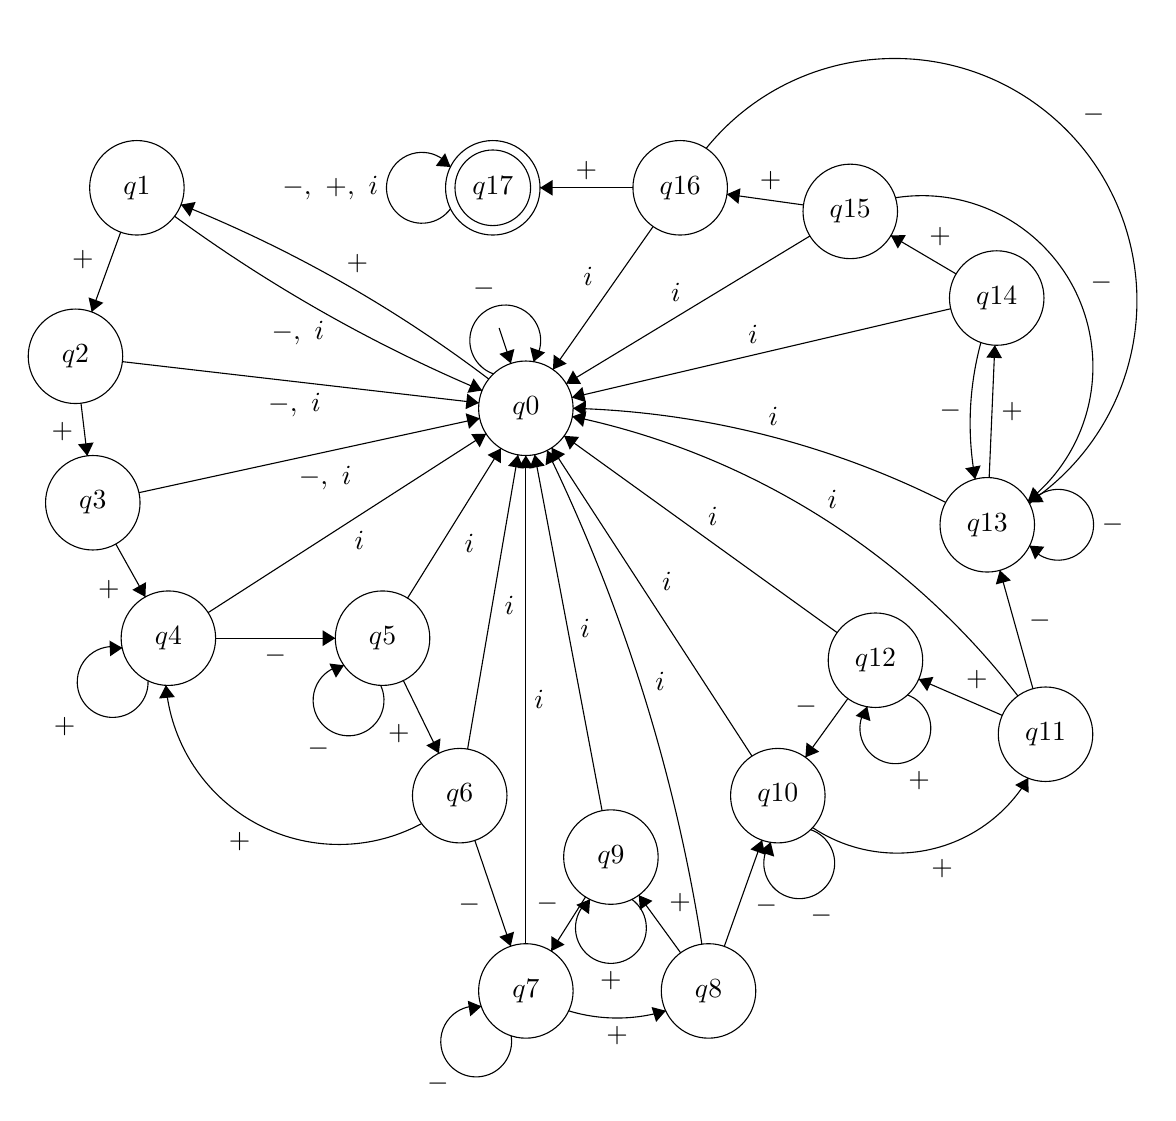
\begin{tikzpicture}[scale=0.2]
\tikzstyle{every node}+=[inner sep=0pt]
\draw [black] (34.2,-17.4) circle (3);
\draw (34.2,-17.4) node {$q0$};
\draw [black] (9.5,-3.4) circle (3);
\draw (9.5,-3.4) node {$q1$};
\draw [black] (5.6,-14.1) circle (3);
\draw (5.6,-14.1) node {$q2$};
\draw [black] (6.7,-23.4) circle (3);
\draw (6.7,-23.4) node {$q3$};
\draw [black] (11.5,-32) circle (3);
\draw (11.5,-32) node {$q4$};
\draw [black] (25.1,-32) circle (3);
\draw (25.1,-32) node {$q5$};
\draw [black] (30,-42) circle (3);
\draw (30,-42) node {$q6$};
\draw [black] (34.2,-54.4) circle (3);
\draw (34.2,-54.4) node {$q7$};
\draw [black] (45.8,-54.4) circle (3);
\draw (45.8,-54.4) node {$q8$};
\draw [black] (39.6,-45.9) circle (3);
\draw (39.6,-45.9) node {$q9$};
\draw [black] (50.2,-42) circle (3);
\draw (50.2,-42) node {$q10$};
\draw [black] (67.2,-38.1) circle (3);
\draw (67.2,-38.1) node {$q11$};
\draw [black] (56.4,-33.4) circle (3);
\draw (56.4,-33.4) node {$q12$};
\draw [black] (63.5,-24.8) circle (3);
\draw (63.5,-24.8) node {$q13$};
\draw [black] (64.1,-10.4) circle (3);
\draw (64.1,-10.4) node {$q14$};
\draw [black] (54.8,-4.9) circle (3);
\draw (54.8,-4.9) node {$q15$};
\draw [black] (44,-3.4) circle (3);
\draw (44,-3.4) node {$q16$};
\draw [black] (32.1,-3.4) circle (3);
\draw (32.1,-3.4) node {$q17$};
\draw [black] (32.1,-3.4) circle (2.4);
\draw [black] (12.303,-4.469) arc (68.10472:52.80601:84.368);
\fill [black] (12.3,-4.47) -- (12.86,-5.23) -- (13.23,-4.3);
\draw (23.5,-8.85) node [above] {$+$};
\draw [black] (31.419,-16.275) arc (-112.91179:-126.17748:97.153);
\fill [black] (31.42,-16.27) -- (30.88,-15.5) -- (30.49,-16.42);
\draw (19.73,-11.81) node [below] {$-,\mbox{ }i$};
\draw [black] (8.47,-6.22) -- (6.63,-11.28);
\fill [black] (6.63,-11.28) -- (7.37,-10.7) -- (6.43,-10.36);
\draw (6.79,-7.96) node [left] {$+$};
\draw [black] (5.95,-17.08) -- (6.35,-20.42);
\fill [black] (6.35,-20.42) -- (6.75,-19.57) -- (5.76,-19.69);
\draw (5.49,-18.87) node [left] {$+$};
\draw [black] (8.16,-26.02) -- (10.04,-29.38);
\fill [black] (10.04,-29.38) -- (10.08,-28.44) -- (9.21,-28.93);
\draw (8.44,-28.91) node [left] {$+$};
\draw [black] (8.58,-14.44) -- (31.22,-17.06);
\fill [black] (31.22,-17.06) -- (30.48,-16.47) -- (30.37,-17.46);
\draw (19.51,-16.39) node [below] {$-,\mbox{ }i$};
\draw [black] (9.63,-22.76) -- (31.27,-18.04);
\fill [black] (31.27,-18.04) -- (30.38,-17.72) -- (30.59,-18.7);
\draw (21.45,-21.03) node [below] {$-,\mbox{ }i$};
\draw [black] (32.155,-15.221) arc (250.91269:-37.08731:2.25);
\draw (31.53,-10.4) node [above] {$-$};
\fill [black] (34.69,-14.45) -- (35.42,-13.86) -- (34.47,-13.53);
\draw [black] (14.5,-32) -- (22.1,-32);
\fill [black] (22.1,-32) -- (21.3,-31.5) -- (21.3,-32.5);
\draw (18.3,-32.5) node [below] {$-$};
\draw [black] (26.42,-34.69) -- (28.68,-39.31);
\fill [black] (28.68,-39.31) -- (28.78,-38.37) -- (27.88,-38.81);
\draw (26.85,-38.09) node [left] {$+$};
\draw [black] (24.974,-34.986) arc (25.32189:-262.67811:2.25);
\draw (21.03,-38.42) node [below] {$-$};
\fill [black] (22.65,-33.72) -- (21.72,-33.61) -- (22.14,-34.51);
\draw [black] (27.588,-43.768) arc (-61.55234:-175.2337:11.03);
\fill [black] (11.34,-34.99) -- (10.91,-35.83) -- (11.91,-35.74);
\draw (16.03,-44.28) node [below] {$+$};
\draw [black] (30.96,-44.84) -- (33.24,-51.56);
\fill [black] (33.24,-51.56) -- (33.45,-50.64) -- (32.51,-50.96);
\draw (31.34,-48.92) node [left] {$-$};
\draw [black] (43.089,-55.662) arc (-73.11558:-106.88442:10.637);
\fill [black] (43.09,-55.66) -- (42.18,-55.42) -- (42.47,-56.37);
\draw (40,-56.62) node [below] {$+$};
\draw [black] (44.03,-51.98) -- (41.37,-48.32);
\fill [black] (41.37,-48.32) -- (41.44,-49.26) -- (42.24,-48.68);
\draw (43.28,-48.77) node [right] {$+$};
\draw [black] (40.923,-48.58) arc (54:-234:2.25);
\draw (39.6,-53.15) node [below] {$+$};
\fill [black] (38.28,-48.58) -- (37.4,-48.93) -- (38.21,-49.52);
\draw [black] (33.264,-57.238) arc (9.47914:-278.52086:2.25);
\draw (28.61,-59.69) node [below] {$-$};
\fill [black] (31.38,-55.38) -- (30.51,-55.02) -- (30.67,-56.01);
\draw [black] (37.99,-48.43) -- (35.81,-51.87);
\fill [black] (35.81,-51.87) -- (36.66,-51.46) -- (35.82,-50.92);
\draw (36.28,-48.85) node [left] {$-$};
\draw [black] (52.27,-44.156) arc (71.56583:-216.43417:2.25);
\draw (52.96,-48.97) node [below] {$-$};
\fill [black] (49.75,-44.95) -- (49.02,-45.55) -- (49.97,-45.87);
\draw [black] (46.8,-51.57) -- (49.2,-44.83);
\fill [black] (49.2,-44.83) -- (48.46,-45.41) -- (49.4,-45.75);
\draw (48.76,-48.96) node [right] {$-$};
\draw [black] (66.103,-40.879) arc (-30.43509:-123.72341:9.668);
\fill [black] (66.1,-40.88) -- (65.27,-41.32) -- (66.13,-41.82);
\draw (60.63,-45.99) node [below] {$+$};
\draw [black] (54.65,-35.83) -- (51.95,-39.57);
\fill [black] (51.95,-39.57) -- (52.83,-39.21) -- (52.02,-38.63);
\draw (52.71,-36.32) node [left] {$-$};
\draw [black] (58.421,-35.601) arc (70.28801:-217.71199:2.25);
\draw (59.17,-40.43) node [below] {$+$};
\fill [black] (55.88,-36.34) -- (55.14,-36.93) -- (56.08,-37.26);
\draw [black] (64.45,-36.9) -- (59.15,-34.6);
\fill [black] (59.15,-34.6) -- (59.68,-35.37) -- (60.08,-34.46);
\draw (62.84,-35.24) node [above] {$+$};
\draw [black] (66.4,-35.21) -- (64.3,-27.69);
\fill [black] (64.3,-27.69) -- (64.04,-28.59) -- (65,-28.33);
\draw (66.12,-30.91) node [right] {$-$};
\draw [black] (66.18,-23.477) arc (144:-144:2.25);
\draw (70.75,-24.8) node [right] {$-$};
\fill [black] (66.18,-26.12) -- (66.53,-27) -- (67.12,-26.19);
\draw [black] (63.62,-21.8) -- (63.98,-13.4);
\fill [black] (63.98,-13.4) -- (63.44,-14.18) -- (64.44,-14.22);
\draw (64.36,-17.62) node [right] {$+$};
\draw [black] (61.52,-8.87) -- (57.38,-6.43);
\fill [black] (57.38,-6.43) -- (57.82,-7.26) -- (58.33,-6.4);
\draw (60.51,-7.15) node [above] {$+$};
\draw [black] (51.83,-4.49) -- (46.97,-3.81);
\fill [black] (46.97,-3.81) -- (47.7,-4.42) -- (47.83,-3.43);
\draw (49.75,-3.55) node [above] {$+$};
\draw [black] (41,-3.4) -- (35.1,-3.4);
\fill [black] (35.1,-3.4) -- (35.9,-3.9) -- (35.9,-2.9);
\draw (38.05,-2.9) node [above] {$+$};
\draw [black] (62.734,-21.902) arc (-169.58588:-195.186:19.603);
\fill [black] (62.73,-21.9) -- (63.08,-21.03) -- (62.1,-21.21);
\draw (61.87,-17.53) node [left] {$-$};
\draw [black] (57.662,-4.033) arc (98.93307:-51.70453:10.861);
\fill [black] (66.08,-23.29) -- (67.02,-23.18) -- (66.4,-22.4);
\draw (70.03,-9.44) node [right] {$-$};
\draw [black] (45.648,-0.899) arc (141.02707:-56.34657:15.391);
\fill [black] (66.14,-23.39) -- (67.09,-23.36) -- (66.53,-22.53);
\draw (69.53,1.25) node [right] {$-$};
\draw [black] (29.42,-4.723) arc (324:36:2.25);
\draw (24.85,-3.4) node [left] {$-,\mbox{ }+,\mbox{ }i$};
\fill [black] (29.42,-2.08) -- (29.07,-1.2) -- (28.48,-2.01);
\draw [black] (32.5,-12.3) -- (33.25,-14.55);
\fill [black] (33.25,-14.55) -- (33.47,-13.64) -- (32.52,-13.95);
\draw [black] (10.21,-34.696) arc (2.15723:-285.84277:2.25);
\draw (5.63,-37.59) node [left] {$+$};
\fill [black] (8.58,-32.62) -- (7.76,-32.15) -- (7.8,-33.15);
\draw [black] (14.02,-30.38) -- (31.68,-19.02);
\fill [black] (31.68,-19.02) -- (30.73,-19.04) -- (31.27,-19.88);
\draw (23.63,-25.2) node [below] {$i$};
\draw [black] (26.69,-29.45) -- (32.61,-19.95);
\fill [black] (32.61,-19.95) -- (31.77,-20.36) -- (32.61,-20.89);
\draw (30.28,-25.99) node [right] {$i$};
\draw [black] (30.5,-39.04) -- (33.7,-20.36);
\fill [black] (33.7,-20.36) -- (33.07,-21.06) -- (34.05,-21.23);
\draw (32.82,-29.94) node [right] {$i$};
\draw [black] (34.2,-51.4) -- (34.2,-20.4);
\fill [black] (34.2,-20.4) -- (33.7,-21.2) -- (34.7,-21.2);
\draw (34.7,-35.9) node [right] {$i$};
\draw [black] (39.04,-42.95) -- (34.76,-20.35);
\fill [black] (34.76,-20.35) -- (34.42,-21.23) -- (35.4,-21.04);
\draw (37.63,-31.36) node [right] {$i$};
\draw [black] (35.547,-20.081) arc (25.90219:8.91163:111.199);
\fill [black] (35.55,-20.08) -- (35.45,-21.02) -- (36.35,-20.58);
\draw (42.39,-34.75) node [right] {$i$};
\draw [black] (48.56,-39.49) -- (35.84,-19.91);
\fill [black] (35.84,-19.91) -- (35.85,-20.86) -- (36.69,-20.31);
\draw (42.82,-28.38) node [right] {$i$};
\draw [black] (53.97,-31.65) -- (36.63,-19.15);
\fill [black] (36.63,-19.15) -- (36.99,-20.03) -- (37.58,-19.22);
\draw (46.08,-24.9) node [above] {$i$};
\draw [black] (37.154,-17.922) arc (78.18431:37.61784:48.167);
\fill [black] (37.15,-17.92) -- (37.83,-18.58) -- (38.04,-17.6);
\draw (53.66,-23.77) node [above] {$i$};
\draw [black] (37.2,-17.403) arc (88.40773:63.24388:56.01);
\fill [black] (37.2,-17.4) -- (37.99,-17.93) -- (38.01,-16.93);
\draw (49.92,-18.53) node [above] {$i$};
\draw [black] (42.28,-5.86) -- (35.92,-14.94);
\fill [black] (35.92,-14.94) -- (36.79,-14.57) -- (35.97,-14);
\draw (38.5,-9.04) node [left] {$i$};
\draw [black] (52.24,-6.46) -- (36.76,-15.84);
\fill [black] (36.76,-15.84) -- (37.71,-15.86) -- (37.19,-15);
\draw (43.72,-10.65) node [above] {$i$};
\draw [black] (61.18,-11.08) -- (37.12,-16.72);
\fill [black] (37.12,-16.72) -- (38.01,-17.02) -- (37.79,-16.05);
\draw (48.63,-13.34) node [above] {$i$};
\end{tikzpicture}
\end{center}

\section{Definició formal de \dfa{}}

Definim formalment el nostre autòmat.

\begin{center}
	\dfa $=$ \{Q, $\Sigma{}$*, $\delta$, q0, q17\}
\end{center}

\begin{itemize}
\item \textbf{Q} = \{q0,q1,q2,q3,q4,q5,q6,q7,q8,q9,q10,q11,q12,q13,q14,q15,q16,q17\}
\item $\Sigma$* $=$ \{ + , - , \Return{} , $\epsilon$ \}
\item $\delta$ $=$ Q X $\Sigma$* $\rightarrow$ Q
\item q0 $\in{}$ Q
\item q17 $\subseteq{}$ Q
\end{itemize}

\subsection{Representació taula $\delta$}

\begin{center}
\begin{table}[ht]
\caption{\label{tab:table-name} $\delta$ table}
\centering
\begin{tabular}{ c c c c }
\hline
\hline
State & +   & -   & \Return   \\ \hline
$\rightarrow$ q0  & q1  & q0  & q0  \\
q1    & q2  & q0  & q0  \\
q2    & q3  & q0  & q0  \\
q3    & q4  & q0  & q0  \\
q4    & q4  & q5  & q0  \\
q5    & q6  & q5  & q0  \\
q6    & q4  & q7  & q0  \\
q7    & q9  & q7  & q0  \\
q8    & q8  & q7  & q0  \\
q9    & q8  & q10 & q0  \\
q10   & q12 & q10 & q0  \\
q11   & q11 & q10 & q0  \\
q12   & q11 & q13 & q0  \\
q13   & q14 & q13 & q0  \\
q14   & q15 & q13 & q0  \\
q15   & q16 & q13 & q0  \\
q16   & q17 & q13 & q0  \\
q17   & q17 & q17 & q17 \\
\hline
\end{tabular}
\end{table}

\end{center}

\section{Operacions regulars amb autòmats}

La definició 1.23 del llibre parla sobre les operacions que es poden realitzar sobre autòmats finits deterministes. En el nostre cas s’ha emprat una tècnica de construcció pel disseny de l’autòmat però es podria emprar una construcció de subautòmats i mitjançant la concatenació dels mateixos (representada amb el caràcter $\bullet$ ) construir el nostre \dfa{}. Hi ha hagut intents de la creació de l’autòmat mitjançant concatenació dels autòmats \dfa$_1$ i \dfa$_2$ intentant dividir el problema en :

\begin{center}
\dfa$_1$ $=$ 4+
\end{center}

\begin{center}
\dfa$_2$ $=$ 3aïllades
\end{center}

on:

\begin{center}
4+ $\bullet$ 3aïllades $\bullet$ 4+
\end{center}

No s’ha seguit per la complexitat de tractar la funcionalitat del RESET, en el cas hipotètic que haguéssim presentat aquest tipus de construcció haguéssim derivat a el conjunt {\dfa$_1$, \dfa$_2$} que concatenat mitjançant l'ús d'un autòmat finit indeterminista s'hauria pogut agrupar en \nfa{}.

\section{Minimització de \dfa{}}

L’objectiu d’aquesta secció és cercar el \dfa{} mínim partint del \dfa{}.

\textbf{Considerem que dos estats fan el mateix si i només si el resultat de les transicions és el mateix considerant tots els símbols de l’alfabet. }

La idea de la minimització parteix de la fusió d'estats. Podem trobar explicats els processos de minimització al document [3]. Podem utilitzar la manera manual aplicant l'algoritme de Hopcroft, o bé, podem optar per utilitzar UTM.

En aquest cas utilitzem l’algoritme de HopCroft per a la seva minimització implementant una matriu que ens permeti detectar les repeticions de les transicions donat un estat.


\begin{center}
\textbf{El nostre autòmat és mínim.}
\end{center}


\begin{table}[ht]
\caption{\label{tab:table-name} Passos de $PI0$ - $PI2$}
\centering
\begin{tabular}{ l l l l l l l l l l l l l l l l l l l l}
\hline
\hline
T      &   & + & - & E & PI0 & + & - & E & PI1 & + & - & E & PI2 &  &  &  &  &  &  \\ \hline
q0  & A & B & A & A & 1   & 1 & 1 & 1 & 1   & 1 & 1 & 1 & 1   &  &  &  &  &  &  \\
q1      & B & C & A & A & 1   & 1 & 1 & 1 & 1   & 1 & 1 & 1 & 1   &  &  &  &  &  &  \\
q2     & C & D & A & A & 1   & 1 & 1 & 1 & 1   & 1 & 1 & 1 & 1   &  &  &  &  &  &  \\
q3    & D & E & A & A & 1   & 1 & 1 & 1 & 1   & 1 & 1 & 1 & 1   &  &  &  &  &  &  \\
q4   & E & E & F & A & 1   & 1 & 1 & 1 & 1   & 1 & 1 & 1 & 1   &  &  &  &  &  &  \\
q5   & F & G & F & A & 1   & 1 & 1 & 1 & 1   & 1 & 1 & 1 & 1   &  &  &  &  &  &  \\
q6   & G & E & H & A & 1   & 1 & 1 & 1 & 1   & 1 & 1 & 1 & 1   &  &  &  &  &  &  \\
q7 & H & J & H & A & 1   & 1 & 1 & 1 & 1   & 1 & 1 & 1 & 1   &  &  &  &  &  &  \\
q8     & I & I & H & A & 1   & 1 & 1 & 1 & 1   & 1 & 1 & 1 & 1   &  &  &  &  &  &  \\
q9   & J & I & K & A & 1   & 1 & 1 & 1 & 1   & 1 & 1 & 1 & 1   &  &  &  &  &  &  \\
q10 & K & M & K & A & 1   & 1 & 1 & 1 & 1   & 1 & 1 & 1 & 1   &  &  &  &  &  &  \\
q11    & L & L & K & A & 1   & 1 & 1 & 1 & 1   & 1 & 1 & 1 & 1   &  &  &  &  &  &  \\
q12   & M & L & N & A & 1   & 1 & 1 & 1 & 1   & 1 & 1 & 1 & 1   &  &  &  &  &  &  \\
q13   & N & O & N & A & 1   & 1 & 1 & 1 & 1   & 1 & 1 & 1 & 1   &  &  &  &  &  &  \\
q14     & O & P & N & A & 1   & 1 & 1 & 1 & 1   & 1 & 1 & 1 & 1   &  &  &  &  &  &  \\
q15    & P & Q & N & A & 1   & 1 & 1 & 1 & 1   & 3 & 1 & 1 & 4   &  &  &  &  &  &  \\
q16   & Q & R & N & A & 1   & 2 & 1 & 1 & 3   & 2 & 1 & 1 & 3   &  &  &  &  &  &  \\
q17  & R & R & R & R & 2   & 2 & 2 & 2 & 2   & 2 & 2 & 2 & 2   &  &  &  &  &  &  \\
       &   &   &   &   &     &   &   &   &     &   &   &   &     &  &  &  &  &  &  \\
       \hline
\end{tabular}
\end{table}


\begin{table}[ht]
\caption{\label{tab:table-name} Passos de $PI3$ - $PI5$}
\centering
\begin{tabular}{ l l l l l l l l l l l l l l l l l l l l }
\hline
\hline
T      & + & - & E & PI3 & + & - & E & PI4 & + & - & E & PI5 &  &  &  &  &  &  &  \\ \hline
q0  & 1 & 1 & 1 & 1   & 1 & 1 & 1 & 1   & 1 & 1 & 1 & 1   &  &  &  &  &  &  &  \\
q1  & 1 & 1 & 1 & 1   & 1 & 1 & 1 & 1   & 1 & 1 & 1 & 1   &  &  &  &  &  &  &  \\
q2  & 1 & 1 & 1 & 1   & 1 & 1 & 1 & 1   & 1 & 1 & 1 & 1   &  &  &  &  &  &  &  \\
q3  & 1 & 1 & 1 & 1   & 1 & 1 & 1 & 1   & 1 & 1 & 1 & 1   &  &  &  &  &  &  &  \\
q4  & 1 & 1 & 1 & 1   & 1 & 1 & 1 & 1   & 1 & 1 & 1 & 1   &  &  &  &  &  &  &  \\
q5  & 1 & 1 & 1 & 1   & 1 & 1 & 1 & 1   & 1 & 1 & 1 & 1   &  &  &  &  &  &  &  \\
q6  & 1 & 1 & 1 & 1   & 1 & 1 & 1 & 1   & 1 & 1 & 1 & 1   &  &  &  &  &  &  &  \\
q7  & 1 & 1 & 1 & 1   & 1 & 1 & 1 & 1   & 1 & 1 & 1 & 1   &  &  &  &  &  &  &  \\
q8  & 1 & 1 & 1 & 1   & 1 & 1 & 1 & 1   & 1 & 1 & 1 & 1   &  &  &  &  &  &  &  \\
q9  & 1 & 1 & 1 & 1   & 1 & 1 & 1 & 1   & 1 & 1 & 1 & 1   &  &  &  &  &  &  &  \\
q10 & 1 & 1 & 1 & 1   & 1 & 1 & 1 & 1   & 1 & 1 & 1 & 1   &  &  &  &  &  &  &  \\
q11 & 1 & 1 & 1 & 1   & 1 & 1 & 1 & 1   & 1 & 1 & 1 & 1   &  &  &  &  &  &  &  \\
q12 & 1 & 1 & 1 & 1   & 1 & 1 & 1 & 1   & 1 & 6 & 1 & 7   &  &  &  &  &  &  &  \\
q13 & 1 & 1 & 1 & 1   & 5 & 1 & 1 & 6   & 5 & 6 & 1 & 6   &  &  &  &  &  &  &  \\
q14 & 4 & 1 & 1 & 5   & 4 & 1 & 1 & 5   & 4 & 6 & 1 & 5   &  &  &  &  &  &  &  \\
q15 & 3 & 1 & 1 & 4   & 3 & 1 & 1 & 4   & 3 & 6 & 1 & 4   &  &  &  &  &  &  &  \\
q16 & 2 & 1 & 1 & 3   & 2 & 1 & 1 & 3   & 2 & 6 & 1 & 3   &  &  &  &  &  &  &  \\
q17 & 2 & 2 & 2 & 2   & 2 & 2 & 2 & 2   & 2 & 2 & 2 & 2   &  &  &  &  &  &  &  \\
       &   &   &   &     &   &   &   &     &   &   &   &     &  &  &  &  &  &  &  \\
       \hline
\end{tabular}
\end{table}

\begin{table}[ht]
\caption{\label{tab:table-name} Passos de $PI9$ - $PI11$}
\centering
\begin{tabular}{ l l l l l l l l l l l l l l l l l l l l }
\hline
\hline
T      & + & - & E & PI6 & + & - & E & PI7 & + & - & E & PI8 &  &  &  &  &  &  &  \\ \hline
q0  & 1 & 1 & 1 & 1   & 1 & 1 & 1 & 1   & 1 & 1 & 1 & 1   &  &  &  &  &  &  &  \\
q1  & 1 & 1 & 1 & 1   & 1 & 1 & 1 & 1   & 1 & 1 & 1 & 1   &  &  &  &  &  &  &  \\
q2  & 1 & 1 & 1 & 1   & 1 & 1 & 1 & 1   & 1 & 1 & 1 & 1   &  &  &  &  &  &  &  \\
q3  & 1 & 1 & 1 & 1   & 1 & 1 & 1 & 1   & 1 & 1 & 1 & 1   &  &  &  &  &  &  &  \\
q4  & 1 & 1 & 1 & 1   & 1 & 1 & 1 & 1   & 1 & 1 & 1 & 1   &  &  &  &  &  &  &  \\
q5  & 1 & 1 & 1 & 1   & 1 & 1 & 1 & 1   & 1 & 1 & 1 & 1   &  &  &  &  &  &  &  \\
q6  & 1 & 1 & 1 & 1   & 1 & 1 & 1 & 1   & 1 & 1 & 1 & 1   &  &  &  &  &  &  &  \\
q7  & 1 & 1 & 1 & 1   & 1 & 1 & 1 & 1   & 9 & 1 & 1 & 11  &  &  &  &  &  &  &  \\
q8  & 1 & 1 & 1 & 1   & 1 & 1 & 1 & 1   & 1 & 1 & 1 & 1   &  &  &  &  &  &  &  \\
q9  & 1 & 1 & 1 & 1   & 1 & 8 & 1 & 9   & 1 & 8 & 1 & 9   &  &  &  &  &  &  &  \\
q10 & 7 & 1 & 1 & 8   & 7 & 8 & 1 & 8   & 7 & 8 & 1 & 8   &  &  &  &  &  &  &  \\
q11 & 1 & 1 & 1 & 1   & 1 & 8 & 1 & 9   & 9 & 8 & 1 & 10  &  &  &  &  &  &  &  \\
q12 & 1 & 6 & 1 & 7   & 1 & 6 & 1 & 7   & 9 & 6 & 1 & 7   &  &  &  &  &  &  &  \\
q13 & 5 & 6 & 1 & 6   & 5 & 6 & 1 & 6   & 5 & 6 & 1 & 6   &  &  &  &  &  &  &  \\
q14 & 4 & 6 & 1 & 5   & 4 & 6 & 1 & 5   & 4 & 6 & 1 & 5   &  &  &  &  &  &  &  \\
q15 & 3 & 6 & 1 & 4   & 3 & 6 & 1 & 4   & 3 & 6 & 1 & 4   &  &  &  &  &  &  &  \\
q16 & 2 & 6 & 1 & 3   & 2 & 6 & 1 & 3   & 2 & 6 & 1 & 3   &  &  &  &  &  &  &  \\
q17 & 2 & 2 & 2 & 2   & 2 & 2 & 2 & 2   & 2 & 2 & 2 & 2   &  &  &  &  &  &  &  \\
       &   &   &   &     &   &   &   &     &   &   &   &     &  &  &  &  &  &  &  \\
       \hline
\end{tabular}
\end{table}


\begin{table}[ht]
\caption{\label{tab:table-name} Passos de $PI12$ - $PI14$}
\centering
\begin{tabular}{ l l l l l l l l l l l l l l l l l l l l }
\hline
\hline
T      & +  & -  & E & PI9 & +  & -  & E & PI10 & +  & -  & E & PI11 &  &  &  &  &  &  &  \\ \hline
q0  & 1  & 1  & 1 & 1   & 1  & 1  & 1 & 1    & 1  & 1  & 1 & 1    &  &  &  &  &  &  &  \\
q1  & 1  & 1  & 1 & 1   & 1  & 1  & 1 & 1    & 1  & 1  & 1 & 1    &  &  &  &  &  &  &  \\
q2  & 1  & 1  & 1 & 1   & 1  & 1  & 1 & 1    & 1  & 1  & 1 & 1    &  &  &  &  &  &  &  \\
q3  & 1  & 1  & 1 & 1   & 1  & 1  & 1 & 1    & 1  & 1  & 1 & 1    &  &  &  &  &  &  &  \\
q4  & 1  & 1  & 1 & 1   & 1  & 1  & 1 & 1    & 1  & 14 & 1 & 15   &  &  &  &  &  &  &  \\
q5  & 1  & 1  & 1 & 1   & 12 & 1  & 1 & 14   & 12 & 14 & 1 & 14   &  &  &  &  &  &  &  \\
q6  & 1  & 11 & 1 & 12  & 1  & 11 & 1 & 12   & 1  & 11 & 1 & 12   &  &  &  &  &  &  &  \\
q7  & 9  & 11 & 1 & 11  & 9  & 11 & 1 & 11   & 9  & 11 & 1 & 11   &  &  &  &  &  &  &  \\
q8  & 1  & 11 & 1 & 12  & 12 & 11 & 1 & 13   & 13 & 11 & 1 & 13   &  &  &  &  &  &  &  \\
q9  & 1  & 8  & 1 & 9   & 12 & 8  & 1 & 9    & 13 & 8  & 1 & 9    &  &  &  &  &  &  &  \\
q10 & 7  & 8  & 1 & 8   & 7  & 8  & 1 & 8    & 7  & 8  & 1 & 8    &  &  &  &  &  &  &  \\
q11 & 10 & 8  & 1 & 10  & 10 & 8  & 1 & 10   & 10 & 8  & 1 & 10   &  &  &  &  &  &  &  \\
q12 & 10 & 6  & 1 & 7   & 10 & 6  & 1 & 7    & 10 & 6  & 1 & 7    &  &  &  &  &  &  &  \\
q13 & 5  & 6  & 1 & 6   & 5  & 6  & 1 & 6    & 5  & 6  & 1 & 6    &  &  &  &  &  &  &  \\
q14 & 4  & 6  & 1 & 5   & 4  & 6  & 1 & 5    & 4  & 6  & 1 & 5    &  &  &  &  &  &  &  \\
q15 & 3  & 6  & 1 & 4   & 3  & 6  & 1 & 4    & 3  & 6  & 1 & 4    &  &  &  &  &  &  &  \\
q16 & 2  & 6  & 1 & 3   & 2  & 6  & 1 & 3    & 2  & 6  & 1 & 3    &  &  &  &  &  &  &  \\
q17 & 2  & 2  & 2 & 2   & 2  & 2  & 2 & 2    & 2  & 2  & 2 & 2    &  &  &  &  &  &  &  \\
       &    &    &   &     &    &    &   &      &    &    &   &      &  &  &  &  &  &  & \\
       \hline
\end{tabular}
\end{table}

\begin{table}[ht]
\caption{\label{tab:table-name} Passos de $PI15$ - $PI16$}
\centering
\begin{tabular}{ l l l l l l l l l l l l l l l l l l l l }
\hline
\hline
T      & +  & -  & E & PI12 & +  & -  & E & PI13 & +  & -  & E & PI14 &  &  &  &  &  &  &  \\ \hline
q0  & 1  & 1  & 1 & 1    & 1  & 1  & 1 & 1    & 1  & 1  & 1 & 1    &  &  &  &  &  &  &  \\
q1  & 1  & 1  & 1 & 1    & 1  & 1  & 1 & 1    & 17 & 1  & 1 & 18   &  &  &  &  &  &  &  \\
q2  & 1  & 1  & 1 & 1    & 16 & 1  & 1 & 17   & 16 & 1  & 1 & 17   &  &  &  &  &  &  &  \\
q3  & 15 & 1  & 1 & 16   & 15 & 1  & 1 & 16   & 15 & 1  & 1 & 16   &  &  &  &  &  &  &  \\
q4  & 15 & 14 & 1 & 15   & 15 & 14 & 1 & 15   & 15 & 14 & 1 & 15   &  &  &  &  &  &  &  \\
q5  & 12 & 14 & 1 & 14   & 12 & 14 & 1 & 14   & 12 & 14 & 1 & 14   &  &  &  &  &  &  &  \\
q6  & 15 & 11 & 1 & 12   & 15 & 11 & 1 & 12   & 15 & 11 & 1 & 12   &  &  &  &  &  &  &  \\
q7  & 9  & 11 & 1 & 11   & 9  & 11 & 1 & 11   & 9  & 11 & 1 & 11   &  &  &  &  &  &  &  \\
q8  & 13 & 11 & 1 & 13   & 13 & 11 & 1 & 13   & 13 & 11 & 1 & 13   &  &  &  &  &  &  &  \\
q9  & 13 & 8  & 1 & 9    & 13 & 8  & 1 & 9    & 13 & 8  & 1 & 9    &  &  &  &  &  &  &  \\
q10 & 7  & 8  & 1 & 8    & 7  & 8  & 1 & 8    & 7  & 8  & 1 & 8    &  &  &  &  &  &  &  \\
q11 & 10 & 8  & 1 & 10   & 10 & 8  & 1 & 10   & 10 & 8  & 1 & 10   &  &  &  &  &  &  &  \\
q12 & 10 & 6  & 1 & 7    & 10 & 6  & 1 & 7    & 10 & 6  & 1 & 7    &  &  &  &  &  &  &  \\
q13 & 5  & 6  & 1 & 6    & 5  & 6  & 1 & 6    & 5  & 6  & 1 & 6    &  &  &  &  &  &  &  \\
q14 & 4  & 6  & 1 & 5    & 4  & 6  & 1 & 5    & 4  & 6  & 1 & 5    &  &  &  &  &  &  &  \\
q15 & 3  & 6  & 1 & 4    & 3  & 6  & 1 & 4    & 3  & 6  & 1 & 4    &  &  &  &  &  &  &  \\
q16 & 2  & 6  & 1 & 3    & 2  & 6  & 1 & 3    & 2  & 6  & 1 & 3    &  &  &  &  &  &  &  \\
q17 & 2  & 2  & 2 & 2    & 2  & 2  & 2 & 2    & 2  & 2  & 2 & 2    &  &  &  &  &  &  &  \\
       &    &    &   &      &    &    &   &      &    &    &   &      &  &  &  &  &  &  & \\
       \hline
\end{tabular}
\end{table}


\begin{table}[ht]
\caption{\label{tab:table-name} Passos de $PI0$ - $PI2$}
\centering
\begin{tabular}{ l l l l l l l l l l l l l l l l l l l l }
\hline
\hline
T      & +  & -  & E & PI15 & +  & -  & E & PI16 &  &  &  &  &  &  &  &  &  &  &  \\
q0  & 18 & 1  & 1 & 1    & 18 & 1  & 1 & 1    &  &  &  &  &  &  &  &  &  &  &  \\
q1  & 17 & 1  & 1 & 18   & 17 & 1  & 1 & 18   &  &  &  &  &  &  &  &  &  &  &  \\
q2  & 16 & 1  & 1 & 17   & 16 & 1  & 1 & 17   &  &  &  &  &  &  &  &  &  &  &  \\
q3  & 15 & 1  & 1 & 16   & 15 & 1  & 1 & 16   &  &  &  &  &  &  &  &  &  &  &  \\
q4  & 15 & 14 & 1 & 15   & 15 & 14 & 1 & 15   &  &  &  &  &  &  &  &  &  &  &  \\
q5  & 12 & 14 & 1 & 14   & 12 & 14 & 1 & 14   &  &  &  &  &  &  &  &  &  &  &  \\
q6  & 15 & 11 & 1 & 12   & 15 & 11 & 1 & 12   &  &  &  &  &  &  &  &  &  &  &  \\
q7  & 9  & 11 & 1 & 11   & 9  & 11 & 1 & 11   &  &  &  &  &  &  &  &  &  &  &  \\
q8  & 13 & 11 & 1 & 13   & 13 & 11 & 1 & 13   &  &  &  &  &  &  &  &  &  &  &  \\
q9  & 13 & 8  & 1 & 9    & 13 & 8  & 1 & 9    &  &  &  &  &  &  &  &  &  &  &  \\
q10 & 7  & 8  & 1 & 8    & 7  & 8  & 1 & 8    &  &  &  &  &  &  &  &  &  &  &  \\
q11 & 10 & 8  & 1 & 10   & 10 & 8  & 1 & 10   &  &  &  &  &  &  &  &  &  &  &  \\
q12 & 10 & 6  & 1 & 7    & 10 & 6  & 1 & 7    &  &  &  &  &  &  &  &  &  &  &  \\
q13 & 5  & 6  & 1 & 6    & 5  & 6  & 1 & 6    &  &  &  &  &  &  &  &  &  &  &  \\
q14 & 4  & 6  & 1 & 5    & 4  & 6  & 1 & 5    &  &  &  &  &  &  &  &  &  &  &  \\
q15 & 3  & 6  & 1 & 4    & 3  & 6  & 1 & 4    &  &  &  &  &  &  &  &  &  &  &  \\
q16 & 2  & 6  & 1 & 3    & 2  & 6  & 1 & 3    &  &  &  &  &  &  &  &  &  &  &  \\
q17 & 2  & 2  & 2 & 2    & 2  & 2  & 2 & 2    &  &  &  &  &  &  &  &  &  &  &  \\ \hline
       &    &    &   &      &    &    &   &      &  &  &  &  &  &  &  &  &  &  &  \\
       \hline
\end{tabular}
\end{table}

\clearpage

\section{NFA (Nondeterministic finit automata)}

L’equivalència de NFA i DFA està demostrada al capítol 1.2 del llibre [1], donat un autòmat NFA existeix un DFA equivalent. Per equivalència entenem que ambdós reconeixen el mateix llenguatge, en aquest cas el llenguatge L(\dfa{}).

Definim doncs \nfa{} com l’autòmat finit indeterminista equivalent a \dfa{}.

\subsection{Disseny de \nfa{}}

Dissenyem \nfa{}, en aquest cas ens convé només cercar el camí que ens porta directes a QAccept. Directament tracem un camí acceptador i el modifiquem perquè es comporti de manera correcta afegint les branques indeterministes oportunes.

\begin{center}
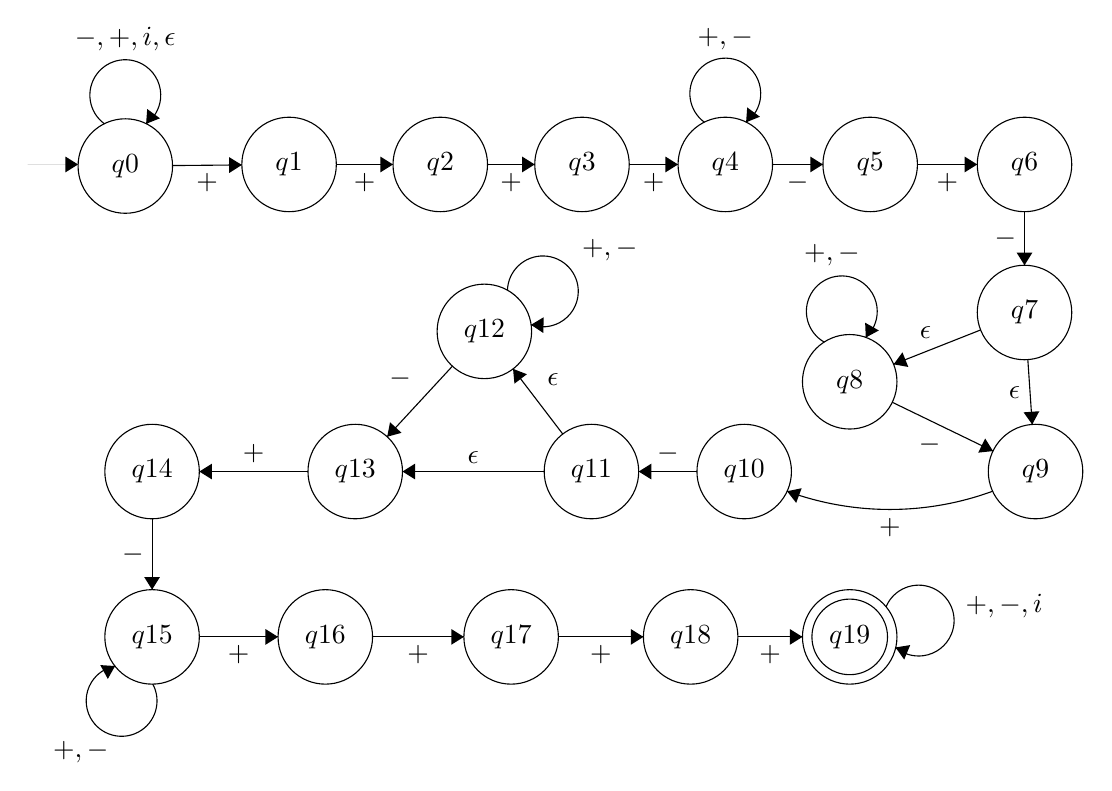
\begin{tikzpicture}[scale=0.2]
\tikzstyle{every node}+=[inner sep=0pt]
\draw [black] (6.2,-11.8) circle (3);
\draw (6.2,-11.8) node {$q0$};
\draw [black] (16.6,-11.7) circle (3);
\draw (16.6,-11.7) node {$q1$};
\draw [black] (26.2,-11.7) circle (3);
\draw (26.2,-11.7) node {$q2$};
\draw [black] (35.2,-11.7) circle (3);
\draw (35.2,-11.7) node {$q3$};
\draw [black] (44.3,-11.7) circle (3);
\draw (44.3,-11.7) node {$q4$};
\draw [black] (53.5,-11.7) circle (3);
\draw (53.5,-11.7) node {$q5$};
\draw [black] (63.3,-11.7) circle (3);
\draw (63.3,-11.7) node {$q6$};
\draw [black] (63.3,-21.1) circle (3);
\draw (63.3,-21.1) node {$q7$};
\draw [black] (52.2,-25.5) circle (3);
\draw (52.2,-25.5) node {$q8$};
\draw [black] (64,-31.2) circle (3);
\draw (64,-31.2) node {$q9$};
\draw [black] (45.5,-31.2) circle (3);
\draw (45.5,-31.2) node {$q10$};
\draw [black] (35.8,-31.2) circle (3);
\draw (35.8,-31.2) node {$q11$};
\draw [black] (29,-22.3) circle (3);
\draw (29,-22.3) node {$q12$};
\draw [black] (20.8,-31.2) circle (3);
\draw (20.8,-31.2) node {$q13$};
\draw [black] (7.9,-31.2) circle (3);
\draw (7.9,-31.2) node {$q14$};
\draw [black] (7.9,-41.7) circle (3);
\draw (7.9,-41.7) node {$q15$};
\draw [black] (18.9,-41.7) circle (3);
\draw (18.9,-41.7) node {$q16$};
\draw [black] (30.7,-41.7) circle (3);
\draw (30.7,-41.7) node {$q17$};
\draw [black] (42.1,-41.7) circle (3);
\draw (42.1,-41.7) node {$q18$};
\draw [black] (52.2,-41.7) circle (3);
\draw (52.2,-41.7) node {$q19$};
\draw [black] (52.2,-41.7) circle (2.4);
\draw [black] (4.877,-9.12) arc (234:-54:2.25);
\draw (6.2,-4.55) node [above] {$-,+,i,\epsilon$};
\fill [black] (7.52,-9.12) -- (8.4,-8.77) -- (7.59,-8.18);
\draw [black] (9.2,-11.77) -- (13.6,-11.73);
\fill [black] (13.6,-11.73) -- (12.8,-11.24) -- (12.8,-12.24);
\draw (11.4,-12.26) node [below] {$+$};
\fill [black] (0,-11.7) -- (2.5,-11.7);
\fill [black] (3.2,-11.7) -- (2.4,-11.2) -- (2.4,-12.2);
\draw [black] (19.6,-11.7) -- (23.2,-11.7);
\fill [black] (23.2,-11.7) -- (22.4,-11.2) -- (22.4,-12.2);
\draw (21.4,-12.2) node [below] {$+$};
\draw [black] (29.2,-11.7) -- (32.2,-11.7);
\fill [black] (32.2,-11.7) -- (31.4,-11.2) -- (31.4,-12.2);
\draw (30.7,-12.2) node [below] {$+$};
\draw [black] (38.2,-11.7) -- (41.3,-11.7);
\fill [black] (41.3,-11.7) -- (40.5,-11.2) -- (40.5,-12.2);
\draw (39.75,-12.2) node [below] {$+$};
\draw [black] (42.977,-9.02) arc (234:-54:2.25);
\draw (44.3,-4.45) node [above] {$+,-$};
\fill [black] (45.62,-9.02) -- (46.5,-8.67) -- (45.69,-8.08);
\draw [black] (47.3,-11.7) -- (50.5,-11.7);
\fill [black] (50.5,-11.7) -- (49.7,-11.2) -- (49.7,-12.2);
\draw (48.9,-12.2) node [below] {$-$};
\draw [black] (56.5,-11.7) -- (60.3,-11.7);
\fill [black] (60.3,-11.7) -- (59.5,-11.2) -- (59.5,-12.2);
\draw (58.4,-12.2) node [below] {$+$};
\draw [black] (63.3,-14.7) -- (63.3,-18.1);
\fill [black] (63.3,-18.1) -- (63.8,-17.3) -- (62.8,-17.3);
\draw (62.8,-16.4) node [left] {$-$};
\draw [black] (63.51,-24.09) -- (63.79,-28.21);
\fill [black] (63.79,-28.21) -- (64.24,-27.37) -- (63.24,-27.44);
\draw (63.05,-26.19) node [left] {$\epsilon$};
\draw [black] (60.51,-22.21) -- (54.99,-24.39);
\fill [black] (54.99,-24.39) -- (55.92,-24.56) -- (55.55,-23.63);
\draw (57.01,-22.79) node [above] {$\epsilon$};
\draw [black] (50.587,-22.984) arc (240.4032:-47.5968:2.25);
\draw (51.07,-18.15) node [above] {$+,-$};
\fill [black] (53.22,-22.69) -- (54.05,-22.24) -- (53.18,-21.75);
\draw [black] (54.9,-26.8) -- (61.3,-29.9);
\fill [black] (61.3,-29.9) -- (60.8,-29.1) -- (60.36,-30);
\draw (57.28,-28.85) node [below] {$-$};
\draw [black] (61.276,-32.45) arc (-69.87784:-110.12216:18.97);
\fill [black] (48.22,-32.45) -- (48.8,-33.19) -- (49.15,-32.26);
\draw (54.75,-34.11) node [below] {$+$};
\draw [black] (42.5,-31.2) -- (38.8,-31.2);
\fill [black] (38.8,-31.2) -- (39.6,-31.7) -- (39.6,-30.7);
\draw (40.65,-30.7) node [above] {$-$};
\draw [black] (33.98,-28.82) -- (30.82,-24.68);
\fill [black] (30.82,-24.68) -- (30.91,-25.62) -- (31.7,-25.02);
\draw (32.97,-25.35) node [right] {$\epsilon$};
\draw [black] (32.8,-31.2) -- (23.8,-31.2);
\fill [black] (23.8,-31.2) -- (24.6,-31.7) -- (24.6,-30.7);
\draw (28.3,-30.7) node [above] {$\epsilon$};
\draw [black] (17.8,-31.2) -- (10.9,-31.2);
\fill [black] (10.9,-31.2) -- (11.7,-31.7) -- (11.7,-30.7);
\draw (14.35,-30.7) node [above] {$+$};
\draw [black] (30.465,-19.696) arc (178.36885:-109.63115:2.25);
\draw (35.17,-17.14) node [right] {$+,-$};
\fill [black] (31.96,-21.88) -- (32.74,-22.4) -- (32.77,-21.4);
\draw [black] (26.97,-24.51) -- (22.83,-28.99);
\fill [black] (22.83,-28.99) -- (23.74,-28.74) -- (23.01,-28.07);
\draw (24.37,-25.29) node [left] {$-$};
\draw [black] (7.9,-34.2) -- (7.9,-38.7);
\fill [black] (7.9,-38.7) -- (8.4,-37.9) -- (7.4,-37.9);
\draw (7.4,-36.45) node [left] {$-$};
\draw [black] (7.941,-44.688) arc (28.51765:-259.48235:2.25);
\draw (3.37,-48.3) node [below] {$+,-$};
\fill [black] (5.55,-43.55) -- (4.61,-43.49) -- (5.09,-44.37);
\draw [black] (10.9,-41.7) -- (15.9,-41.7);
\fill [black] (15.9,-41.7) -- (15.1,-41.2) -- (15.1,-42.2);
\draw (13.4,-42.2) node [below] {$+$};
\draw [black] (21.9,-41.7) -- (27.7,-41.7);
\fill [black] (27.7,-41.7) -- (26.9,-41.2) -- (26.9,-42.2);
\draw (24.8,-42.2) node [below] {$+$};
\draw [black] (33.7,-41.7) -- (39.1,-41.7);
\fill [black] (39.1,-41.7) -- (38.3,-41.2) -- (38.3,-42.2);
\draw (36.4,-42.2) node [below] {$+$};
\draw [black] (45.1,-41.7) -- (49.2,-41.7);
\fill [black] (49.2,-41.7) -- (48.4,-41.2) -- (48.4,-42.2);
\draw (47.15,-42.2) node [below] {$+$};
\draw [black] (54.503,-39.796) arc (157.30497:-130.69503:2.25);
\draw (59.52,-39.73) node [right] {$+,-,i$};
\fill [black] (55.11,-42.37) -- (55.66,-43.14) -- (56.04,-42.22);
\end{tikzpicture}
\end{center}


\section{Definició formal de \nfa{}}

Definim formalment el nostre autòmat.

\begin{center}
	\dfa $=$ \{Q, $\Sigma{}$*, $\delta$, q0, q19\}
\end{center}

\begin{itemize}
\item \textbf{Q} = \{q0,q1,q2,q3,q4,q5,q6,q7,q8,q9,q10,q11,q12,q13,q14,q15,q16,q17,q18,q19\}
\item $\Sigma$* $=$ \{ + , - , \Return{} , $\epsilon$ \}
\item $\delta$ $=$ Q X $\Sigma$* $\rightarrow$ P(Q) on P(Q)sónpossibles subconjunts de Q
\item q0 $\in{}$ Q
\item q19 $\subseteq{}$ Q
\end{itemize}


\subsection{Representació taula $\delta$}

\begin{center}
\begin{table}[ht]
\caption{\label{tab:table-name} $\delta$ table}
\centering
\begin{tabular}{ l l l l l l l l l l l l l l l l l l l l }
\hline
\hline
State & +           & -           & \Return & $\epsilon$              &  &  &  &  &  &  &  &  &  &  &  &  &  &  &  \\ \hline
q0    & \{q0,q1\}   & \{q0\}      & \{q0\}                 & \{q0\}                  &  &  &  &  &  &  &  &  &  &  &  &  &  &  &  \\
q1    & \{q2\}      & $\emptyset$ & $\emptyset$            & $\emptyset$             &  &  &  &  &  &  &  &  &  &  &  &  &  &  &  \\
q2    & \{q3\}      & $\emptyset$ & $\emptyset$            & $\emptyset$             &  &  &  &  &  &  &  &  &  &  &  &  &  &  &  \\
q3    & \{q4\}      & $\emptyset$ & $\emptyset$            & $\emptyset$             &  &  &  &  &  &  &  &  &  &  &  &  &  &  &  \\
q4    & \{q4\}      & \{q4,q5\}   & $\emptyset$            & $\emptyset$             &  &  &  &  &  &  &  &  &  &  &  &  &  &  &  \\
q5    & \{q6\}      & $\emptyset$ & $\emptyset$            & $\emptyset$             &  &  &  &  &  &  &  &  &  &  &  &  &  &  &  \\
q6    & $\emptyset$ & \{q7\}      & $\emptyset$            & $\emptyset$             &  &  &  &  &  &  &  &  &  &  &  &  &  &  &  \\
q7    & $\emptyset$ & $\emptyset$ & $\emptyset$            & \{q8,q9\}               &  &  &  &  &  &  &  &  &  &  &  &  &  &  &  \\
q8    & \{q8\}      & \{q8,q9\}   & $\emptyset$            & $\emptyset$             &  &  &  &  &  &  &  &  &  &  &  &  &  &  &  \\
q9    & \{q10\}     & $\emptyset$ & $\emptyset$            & $\emptyset$             &  &  &  &  &  &  &  &  &  &  &  &  &  &  &  \\
q10   & $\emptyset$ & \{q11\}     & $\emptyset$            & $\emptyset$             &  &  &  &  &  &  &  &  &  &  &  &  &  &  &  \\
q11   & $\emptyset$ & $\emptyset$ & $\emptyset$            & \{q12,q13\}             &  &  &  &  &  &  &  &  &  &  &  &  &  &  &  \\
q12   & \{q12\}     & \{q12,q13\} & $\emptyset$            & $\emptyset$             &  &  &  &  &  &  &  &  &  &  &  &  &  &  &  \\
q13   & \{q14\}     & $\emptyset$ & $\emptyset$            & $\emptyset$             &  &  &  &  &  &  &  &  &  &  &  &  &  &  &  \\
q14   & $\emptyset$ & \{q15\}     & $\emptyset$            & $\emptyset$             &  &  &  &  &  &  &  &  &  &  &  &  &  &  &  \\
q15   & \{q15,q16\} & \{q15\}     & $\emptyset$            & $\emptyset$             &  &  &  &  &  &  &  &  &  &  &  &  &  &  &  \\
q16   & \{q17\}     & $\emptyset$ & $\emptyset$            & $\emptyset$             &  &  &  &  &  &  &  &  &  &  &  &  &  &  &  \\
q17   & \{q18\}     & $\emptyset$ & $\emptyset$            & $\emptyset$             &  &  &  &  &  &  &  &  &  &  &  &  &  &  &  \\
q18   & \{q19\}     & $\emptyset$ & $\emptyset$            & $\emptyset$             &  &  &  &  &  &  &  &  &  &  &  &  &  &  &  \\
q19   & \{q19\}     & \{q19\}     & \{q19\}                & $\emptyset$ &  &  &  &  &  &  &  &  &  &  &  &  &  &  & \\ \hline

\end{tabular}
\end{table}

\end{center}

\subsection{Demostrem l’equivalència de \nfa{} i \dfa{}}

Per demostrar l’equivalència dels autòmats apliquem un procés de determinització sobre \nfa{} obtenint \dfa{}'. Ens ajudem de \textit{UTM veure referència [4]}.

Expressem l’autòmat en format UTM mitjançant un fitxer .def tenint en compte que UTM contempla alfabets $\Sigma$*

\begin{lstlisting}

Sigma=[-+i]
Final=[q19]
--------------------
| Description: ANFA
|   Sigma = {-,+,i}
|   L = "exists the sequence '-+-' 3 times flanked both sides by the sequence '++++'"
| Function: f : Sigma^* -> Boolean
|   f(w) = 1, if word in L
|        = 0, otherwise
| Input: word w (e.g., ----+-+-+-+-+-+++-----+i++++---+-+-+++---+-++++i----+-+-+-+-+-+++-----+i)
|   where i = \Return
| Output: 0 or 1
| Date: November, 2018
| Version: 1.0
| UTM-version: 0.2357111317192329313741434753
| Author: Copyright 2011 Gil Gasso Rovira, Marc Sanchez Pifarre, Francesc Xavier Bullich Parra
--------------------------------------------------------------
[q0|-]=[q0]
[q0|+]=[q0]
[q0|i]=[q0]
[q0|.]=[q0]
[q0|+]=[q1]
[q1|+]=[q2]
[q2|+]=[q3]
[q3|+]=[q4]
[q4|+]=[q4]
[q4|-]=[q4]
[q4|-]=[q5]
[q5|+]=[q6]
[q6|-]=[q7]
[q7|.]=[q8]
[q7|.]=[q9]
[q8|+]=[q8]
[q8|-]=[q8]
[q8|-]=[q9]
[q9|+]=[q10]
[q10|-]=[q11]
[q11|.]=[q12]
[q11|.]=[q13]
[q12|+]=[q12]
[q12|-]=[q12]
[q12|-]=[q13]
[q13|+]=[q14]
[q14|-]=[q15]
[q15|-]=[q15]
[q15|+]=[q15]
[q15|+]=[q16]
[q16|+]=[q17]
[q17|+]=[q18]
[q18|+]=[q19]
[q19|+]=[q19]
[q19|-]=[q19]
[q19|i]=[q19]


\end{lstlisting}

Aplicant el procés de determinització que permet UTM obtenim \dfa{}' on \dfa{}' Comprés dins del DFA. Tenir en compte que tal com comenta la \textit{PROOF IDEA de la pàgina 55 de la referència [1]}, NFA de k estats es pot determinitzar en un DFA de $n^k$ estats, és per aquest motiu que la següent representació pot semblar monstruosa.

\begin{lstlisting}
==========================================
| Description: ADFA
|   Sigma = {-,+,i}
|   L = "exists the sequence '-+-' 3 times flanked both sides by the sequence '++++'"
| Function: f : Sigma^* -> Boolean
|   f(w) = 1, if word in L
|        = 0, otherwise
| Input: word w (e.g., ----+-+-+-+-+-+++-----+i++++---+-+-+++---+-++++i----+-+-+-+-+-+++-----+i)
|   where i = \Return
| Output: 0 or 1
| Date: November, 2018
| Version: 1.0
| UTM-version: 0.2357111317192329313741434753
| Author: Copyright 2011 Gil Gasso Rovira, Marc Sanchez Pifarre, Francesc Xavier Bullich Parra
==========================================
Q = {{q1, q8, q6, q12, q10, q14, q15, q4, q16, q19, q0}, {q1, q8, q6, q12, q10, q14, q15, q4, q16, q0}, {q1, q8, q6, q12, q10, q14, q4, q19, q0}, {q1, q8, q6, q12, q10, q14, q4, q0}, {q1, q8, q6, q10, q4, q19, q0}, {q1, q8, q6, q10, q4, q0}, {q1, q8, q2, q12, q3, q15, q4, q16, q17, q18, q19, q0}, {q1, q8, q2, q12, q3, q15, q4, q16, q17, q18, q0}, {q1, q8, q2, q12, q3, q4, q19, q0}, {q1, q8, q2, q12, q3, q4, q0}, {q1, q8, q2, q12, q15, q4, q16, q17, q19, q0}, {q1, q8, q2, q12, q15, q4, q16, q17, q0}, {q1, q8, q2, q12, q4, q19, q0}, {q1, q8, q2, q12, q4, q0}, {q1, q8, q2, q3, q4, q19, q0}, {q1, q8, q2, q3, q4, q0}, {q1, q8, q2, q4, q19, q0}, {q1, q8, q2, q4, q0}, {q1, q6, q4, q19, q0}, {q1, q6, q4, q0}, {q1, q2, q3, q4, q19, q0}, {q1, q2, q3, q4, q0}, {q1, q2, q3, q19, q0}, {q1, q2, q3, q0}, {q1, q2, q4, q19, q0}, {q1, q2, q4, q0}, {q1, q2, q19, q0}, {q1, q2, q0}, {q1, q19, q0}, {q1, q0}, {q8, q5, q7, q12, q9, q11, q13, q15, q4, q19, q0}, {q8, q5, q7, q12, q9, q11, q13, q15, q4, q0}, {q8, q5, q7, q12, q9, q11, q13, q4, q19, q0}, {q8, q5, q7, q12, q9, q11, q13, q4, q0}, {q8, q5, q7, q9, q4, q19, q0}, {q8, q5, q7, q9, q4, q0}, {q8, q5, q12, q9, q13, q15, q4, q19, q0}, {q8, q5, q12, q9, q13, q15, q4, q0}, {q8, q5, q12, q9, q13, q4, q19, q0}, {q8, q5, q12, q9, q13, q4, q0}, {q8, q5, q9, q4, q19, q0}, {q8, q5, q9, q4, q0}, {q5, q4, q19, q0}, {q5, q4, q0}, {q19, q0}, {q0}}
Sigma = {+, -, i}
Initial state = {q0}
Final = {{q1, q8, q6, q12, q10, q14, q15, q4, q16, q19, q0}, {q1, q8, q6, q12, q10, q14, q4, q19, q0}, {q1, q8, q6, q10, q4, q19, q0}, {q1, q8, q2, q12, q3, q15, q4, q16, q17, q18, q19, q0}, {q1, q8, q2, q12, q3, q4, q19, q0}, {q1, q8, q2, q12, q15, q4, q16, q17, q19, q0}, {q1, q8, q2, q12, q4, q19, q0}, {q1, q8, q2, q3, q4, q19, q0}, {q1, q8, q2, q4, q19, q0}, {q1, q6, q4, q19, q0}, {q1, q2, q3, q4, q19, q0}, {q1, q2, q3, q19, q0}, {q1, q2, q4, q19, q0}, {q1, q2, q19, q0}, {q1, q19, q0}, {q8, q5, q7, q12, q9, q11, q13, q15, q4, q19, q0}, {q8, q5, q7, q12, q9, q11, q13, q4, q19, q0}, {q8, q5, q7, q9, q4, q19, q0}, {q8, q5, q12, q9, q13, q15, q4, q19, q0}, {q8, q5, q12, q9, q13, q4, q19, q0}, {q8, q5, q9, q4, q19, q0}, {q5, q4, q19, q0}, {q19, q0}}
==========================================
delta({q1, q8, q6, q12, q10, q14, q15, q4, q16, q19, q0}, +) = {{q1, q8, q2, q12, q15, q4, q16, q17, q19, q0}}
delta({q1, q8, q6, q12, q10, q14, q15, q4, q16, q19, q0}, -) = {{q8, q5, q7, q12, q9, q11, q13, q15, q4, q19, q0}}
delta({q1, q8, q6, q12, q10, q14, q15, q4, q16, q19, q0}, i) = {{q19, q0}}
delta({q1, q8, q6, q12, q10, q14, q15, q4, q16, q0}, +) = {{q1, q8, q2, q12, q15, q4, q16, q17, q0}}
delta({q1, q8, q6, q12, q10, q14, q15, q4, q16, q0}, -) = {{q8, q5, q7, q12, q9, q11, q13, q15, q4, q0}}
delta({q1, q8, q6, q12, q10, q14, q15, q4, q16, q0}, i) = {{q0}}
delta({q1, q8, q6, q12, q10, q14, q4, q19, q0}, +) = {{q1, q8, q2, q12, q4, q19, q0}}
delta({q1, q8, q6, q12, q10, q14, q4, q19, q0}, -) = {{q8, q5, q7, q12, q9, q11, q13, q15, q4, q19, q0}}
delta({q1, q8, q6, q12, q10, q14, q4, q19, q0}, i) = {{q19, q0}}
delta({q1, q8, q6, q12, q10, q14, q4, q0}, +) = {{q1, q8, q2, q12, q4, q0}}
delta({q1, q8, q6, q12, q10, q14, q4, q0}, -) = {{q8, q5, q7, q12, q9, q11, q13, q15, q4, q0}}
delta({q1, q8, q6, q12, q10, q14, q4, q0}, i) = {{q0}}
delta({q1, q8, q6, q10, q4, q19, q0}, +) = {{q1, q8, q2, q4, q19, q0}}
delta({q1, q8, q6, q10, q4, q19, q0}, -) = {{q8, q5, q7, q12, q9, q11, q13, q4, q19, q0}}
delta({q1, q8, q6, q10, q4, q19, q0}, i) = {{q19, q0}}
delta({q1, q8, q6, q10, q4, q0}, +) = {{q1, q8, q2, q4, q0}}
delta({q1, q8, q6, q10, q4, q0}, -) = {{q8, q5, q7, q12, q9, q11, q13, q4, q0}}
delta({q1, q8, q6, q10, q4, q0}, i) = {{q0}}
delta({q1, q8, q2, q12, q3, q15, q4, q16, q17, q18, q19, q0}, +) = {{q1, q8, q2, q12, q3, q15, q4, q16, q17, q18, q19, q0}}
delta({q1, q8, q2, q12, q3, q15, q4, q16, q17, q18, q19, q0}, -) = {{q8, q5, q12, q9, q13, q15, q4, q19, q0}}
delta({q1, q8, q2, q12, q3, q15, q4, q16, q17, q18, q19, q0}, i) = {{q19, q0}}
delta({q1, q8, q2, q12, q3, q15, q4, q16, q17, q18, q0}, +) = {{q1, q8, q2, q12, q3, q15, q4, q16, q17, q18, q19, q0}}
delta({q1, q8, q2, q12, q3, q15, q4, q16, q17, q18, q0}, -) = {{q8, q5, q12, q9, q13, q15, q4, q0}}
delta({q1, q8, q2, q12, q3, q15, q4, q16, q17, q18, q0}, i) = {{q0}}
delta({q1, q8, q2, q12, q3, q4, q19, q0}, +) = {{q1, q8, q2, q12, q3, q4, q19, q0}}
delta({q1, q8, q2, q12, q3, q4, q19, q0}, -) = {{q8, q5, q12, q9, q13, q4, q19, q0}}
delta({q1, q8, q2, q12, q3, q4, q19, q0}, i) = {{q19, q0}}
delta({q1, q8, q2, q12, q3, q4, q0}, +) = {{q1, q8, q2, q12, q3, q4, q0}}
delta({q1, q8, q2, q12, q3, q4, q0}, -) = {{q8, q5, q12, q9, q13, q4, q0}}
delta({q1, q8, q2, q12, q3, q4, q0}, i) = {{q0}}
delta({q1, q8, q2, q12, q15, q4, q16, q17, q19, q0}, +) = {{q1, q8, q2, q12, q3, q15, q4, q16, q17, q18, q19, q0}}
delta({q1, q8, q2, q12, q15, q4, q16, q17, q19, q0}, -) = {{q8, q5, q12, q9, q13, q15, q4, q19, q0}}
delta({q1, q8, q2, q12, q15, q4, q16, q17, q19, q0}, i) = {{q19, q0}}
delta({q1, q8, q2, q12, q15, q4, q16, q17, q0}, +) = {{q1, q8, q2, q12, q3, q15, q4, q16, q17, q18, q0}}
delta({q1, q8, q2, q12, q15, q4, q16, q17, q0}, -) = {{q8, q5, q12, q9, q13, q15, q4, q0}}
delta({q1, q8, q2, q12, q15, q4, q16, q17, q0}, i) = {{q0}}
delta({q1, q8, q2, q12, q4, q19, q0}, +) = {{q1, q8, q2, q12, q3, q4, q19, q0}}
delta({q1, q8, q2, q12, q4, q19, q0}, -) = {{q8, q5, q12, q9, q13, q4, q19, q0}}
delta({q1, q8, q2, q12, q4, q19, q0}, i) = {{q19, q0}}
delta({q1, q8, q2, q12, q4, q0}, +) = {{q1, q8, q2, q12, q3, q4, q0}}
delta({q1, q8, q2, q12, q4, q0}, -) = {{q8, q5, q12, q9, q13, q4, q0}}
delta({q1, q8, q2, q12, q4, q0}, i) = {{q0}}
delta({q1, q8, q2, q3, q4, q19, q0}, +) = {{q1, q8, q2, q3, q4, q19, q0}}
delta({q1, q8, q2, q3, q4, q19, q0}, -) = {{q8, q5, q9, q4, q19, q0}}
delta({q1, q8, q2, q3, q4, q19, q0}, i) = {{q19, q0}}
delta({q1, q8, q2, q3, q4, q0}, +) = {{q1, q8, q2, q3, q4, q0}}
delta({q1, q8, q2, q3, q4, q0}, -) = {{q8, q5, q9, q4, q0}}
delta({q1, q8, q2, q3, q4, q0}, i) = {{q0}}
delta({q1, q8, q2, q4, q19, q0}, +) = {{q1, q8, q2, q3, q4, q19, q0}}
delta({q1, q8, q2, q4, q19, q0}, -) = {{q8, q5, q9, q4, q19, q0}}
delta({q1, q8, q2, q4, q19, q0}, i) = {{q19, q0}}
delta({q1, q8, q2, q4, q0}, +) = {{q1, q8, q2, q3, q4, q0}}
delta({q1, q8, q2, q4, q0}, -) = {{q8, q5, q9, q4, q0}}
delta({q1, q8, q2, q4, q0}, i) = {{q0}}
delta({q1, q6, q4, q19, q0}, +) = {{q1, q2, q4, q19, q0}}
delta({q1, q6, q4, q19, q0}, -) = {{q8, q5, q7, q9, q4, q19, q0}}
delta({q1, q6, q4, q19, q0}, i) = {{q19, q0}}
delta({q1, q6, q4, q0}, +) = {{q1, q2, q4, q0}}
delta({q1, q6, q4, q0}, -) = {{q8, q5, q7, q9, q4, q0}}
delta({q1, q6, q4, q0}, i) = {{q0}}
delta({q1, q2, q3, q4, q19, q0}, +) = {{q1, q2, q3, q4, q19, q0}}
delta({q1, q2, q3, q4, q19, q0}, -) = {{q5, q4, q19, q0}}
delta({q1, q2, q3, q4, q19, q0}, i) = {{q19, q0}}
delta({q1, q2, q3, q4, q0}, +) = {{q1, q2, q3, q4, q0}}
delta({q1, q2, q3, q4, q0}, -) = {{q5, q4, q0}}
delta({q1, q2, q3, q4, q0}, i) = {{q0}}
delta({q1, q2, q3, q19, q0}, +) = {{q1, q2, q3, q4, q19, q0}}
delta({q1, q2, q3, q19, q0}, -) = {{q19, q0}}
delta({q1, q2, q3, q19, q0}, i) = {{q19, q0}}
delta({q1, q2, q3, q0}, +) = {{q1, q2, q3, q4, q0}}
delta({q1, q2, q3, q0}, -) = {{q0}}
delta({q1, q2, q3, q0}, i) = {{q0}}
delta({q1, q2, q4, q19, q0}, +) = {{q1, q2, q3, q4, q19, q0}}
delta({q1, q2, q4, q19, q0}, -) = {{q5, q4, q19, q0}}
delta({q1, q2, q4, q19, q0}, i) = {{q19, q0}}
delta({q1, q2, q4, q0}, +) = {{q1, q2, q3, q4, q0}}
delta({q1, q2, q4, q0}, -) = {{q5, q4, q0}}
delta({q1, q2, q4, q0}, i) = {{q0}}
delta({q1, q2, q19, q0}, +) = {{q1, q2, q3, q19, q0}}
delta({q1, q2, q19, q0}, -) = {{q19, q0}}
delta({q1, q2, q19, q0}, i) = {{q19, q0}}
delta({q1, q2, q0}, +) = {{q1, q2, q3, q0}}
delta({q1, q2, q0}, -) = {{q0}}
delta({q1, q2, q0}, i) = {{q0}}
delta({q1, q19, q0}, +) = {{q1, q2, q19, q0}}
delta({q1, q19, q0}, -) = {{q19, q0}}
delta({q1, q19, q0}, i) = {{q19, q0}}
delta({q1, q0}, +) = {{q1, q2, q0}}
delta({q1, q0}, -) = {{q0}}
delta({q1, q0}, i) = {{q0}}
delta({q8, q5, q7, q12, q9, q11, q13, q15, q4, q19, q0}, +) = {{q1, q8, q6, q12, q10, q14, q15, q4, q16, q19, q0}}
delta({q8, q5, q7, q12, q9, q11, q13, q15, q4, q19, q0}, -) = {{q8, q5, q12, q9, q13, q15, q4, q19, q0}}
delta({q8, q5, q7, q12, q9, q11, q13, q15, q4, q19, q0}, i) = {{q19, q0}}
delta({q8, q5, q7, q12, q9, q11, q13, q15, q4, q0}, +) = {{q1, q8, q6, q12, q10, q14, q15, q4, q16, q0}}
delta({q8, q5, q7, q12, q9, q11, q13, q15, q4, q0}, -) = {{q8, q5, q12, q9, q13, q15, q4, q0}}
delta({q8, q5, q7, q12, q9, q11, q13, q15, q4, q0}, i) = {{q0}}
delta({q8, q5, q7, q12, q9, q11, q13, q4, q19, q0}, +) = {{q1, q8, q6, q12, q10, q14, q4, q19, q0}}
delta({q8, q5, q7, q12, q9, q11, q13, q4, q19, q0}, -) = {{q8, q5, q12, q9, q13, q4, q19, q0}}
delta({q8, q5, q7, q12, q9, q11, q13, q4, q19, q0}, i) = {{q19, q0}}
delta({q8, q5, q7, q12, q9, q11, q13, q4, q0}, +) = {{q1, q8, q6, q12, q10, q14, q4, q0}}
delta({q8, q5, q7, q12, q9, q11, q13, q4, q0}, -) = {{q8, q5, q12, q9, q13, q4, q0}}
delta({q8, q5, q7, q12, q9, q11, q13, q4, q0}, i) = {{q0}}
delta({q8, q5, q7, q9, q4, q19, q0}, +) = {{q1, q8, q6, q10, q4, q19, q0}}
delta({q8, q5, q7, q9, q4, q19, q0}, -) = {{q8, q5, q9, q4, q19, q0}}
delta({q8, q5, q7, q9, q4, q19, q0}, i) = {{q19, q0}}
delta({q8, q5, q7, q9, q4, q0}, +) = {{q1, q8, q6, q10, q4, q0}}
delta({q8, q5, q7, q9, q4, q0}, -) = {{q8, q5, q9, q4, q0}}
delta({q8, q5, q7, q9, q4, q0}, i) = {{q0}}
delta({q8, q5, q12, q9, q13, q15, q4, q19, q0}, +) = {{q1, q8, q6, q12, q10, q14, q15, q4, q16, q19, q0}}
delta({q8, q5, q12, q9, q13, q15, q4, q19, q0}, -) = {{q8, q5, q12, q9, q13, q15, q4, q19, q0}}
delta({q8, q5, q12, q9, q13, q15, q4, q19, q0}, i) = {{q19, q0}}
delta({q8, q5, q12, q9, q13, q15, q4, q0}, +) = {{q1, q8, q6, q12, q10, q14, q15, q4, q16, q0}}
delta({q8, q5, q12, q9, q13, q15, q4, q0}, -) = {{q8, q5, q12, q9, q13, q15, q4, q0}}
delta({q8, q5, q12, q9, q13, q15, q4, q0}, i) = {{q0}}
delta({q8, q5, q12, q9, q13, q4, q19, q0}, +) = {{q1, q8, q6, q12, q10, q14, q4, q19, q0}}
delta({q8, q5, q12, q9, q13, q4, q19, q0}, -) = {{q8, q5, q12, q9, q13, q4, q19, q0}}
delta({q8, q5, q12, q9, q13, q4, q19, q0}, i) = {{q19, q0}}
delta({q8, q5, q12, q9, q13, q4, q0}, +) = {{q1, q8, q6, q12, q10, q14, q4, q0}}
delta({q8, q5, q12, q9, q13, q4, q0}, -) = {{q8, q5, q12, q9, q13, q4, q0}}
delta({q8, q5, q12, q9, q13, q4, q0}, i) = {{q0}}
delta({q8, q5, q9, q4, q19, q0}, +) = {{q1, q8, q6, q10, q4, q19, q0}}
delta({q8, q5, q9, q4, q19, q0}, -) = {{q8, q5, q9, q4, q19, q0}}
delta({q8, q5, q9, q4, q19, q0}, i) = {{q19, q0}}
delta({q8, q5, q9, q4, q0}, +) = {{q1, q8, q6, q10, q4, q0}}
delta({q8, q5, q9, q4, q0}, -) = {{q8, q5, q9, q4, q0}}
delta({q8, q5, q9, q4, q0}, i) = {{q0}}
delta({q5, q4, q19, q0}, +) = {{q1, q6, q4, q19, q0}}
delta({q5, q4, q19, q0}, -) = {{q5, q4, q19, q0}}
delta({q5, q4, q19, q0}, i) = {{q19, q0}}
delta({q5, q4, q0}, +) = {{q1, q6, q4, q0}}
delta({q5, q4, q0}, -) = {{q5, q4, q0}}
delta({q5, q4, q0}, i) = {{q0}}
delta({q19, q0}, +) = {{q1, q19, q0}}
delta({q19, q0}, -) = {{q19, q0}}
delta({q19, q0}, i) = {{q19, q0}}
delta({q0}, +) = {{q1, q0}}
delta({q0}, -) = {{q0}}
delta({q0}, i) = {{q0}}
==========================================


End DFA definition
==========================================

\end{lstlisting}

Per poder verificar que els dos autòmats reconeixen el mateix llenguatge i per treballar amb autòmats més manejables emprem la minimització explicada a l’apartat \textit{2.5 Minimització de \dfa{}} per minimitzar \dfa{}', concretament s’utilitza la sortida generada per UTM anomenat mfa.def que representa l’autòmat finit determinista mínim.

\begin{lstlisting}

==========================================
| Description: ANFA
|   Sigma = {-,+,i}
|   L = "exists the sequence '-+-' 3 times flanked both sides by the sequence '++++'"
| Function: f : Sigma^* -> Boolean
|   f(w) = 1, if word in L
|        = 0, otherwise
| Input: word w (e.g., ----+-+-+-+-+-+++-----+i++++---+-+-+++---+-++++i----+-+-+-+-+-+++-----+i)
|   where i = \Return
| Output: 0 or 1
| Date: November, 2018
| Version: 1.0
| UTM-version: 0.2357111317192329313741434753
| Author: Copyright 2011 Gil Gasso Rovira, Marc Sanchez Pifarre, Francesc Xavier Bullich Parra
==========================================
Q = {1, 10, 11, 12, 13, 14, 15, 16, 17, 18, 2, 3, 4, 5, 6, 7, 8, 9}
Sigma = {+, -, i}
Initial state = 1
Final = {3}
==========================================
delta(1, +) = {14}
delta(1, -) = {1}
delta(1, i) = {1}
delta(10, +) = {11}
delta(10, -) = {17}
delta(10, i) = {1}
delta(11, +) = {11}
delta(11, -) = {18}
delta(11, i) = {1}
delta(12, +) = {11}
delta(12, -) = {1}
delta(12, i) = {1}
delta(13, +) = {12}
delta(13, -) = {1}
delta(13, i) = {1}
delta(14, +) = {13}
delta(14, -) = {1}
delta(14, i) = {1}
delta(15, +) = {2}
delta(15, -) = {15}
delta(15, i) = {1}
delta(16, +) = {4}
delta(16, -) = {16}
delta(16, i) = {1}
delta(17, +) = {5}
delta(17, -) = {17}
delta(17, i) = {1}
delta(18, +) = {10}
delta(18, -) = {18}
delta(18, i) = {1}
delta(2, +) = {8}
delta(2, -) = {15}
delta(2, i) = {1}
delta(3, +) = {3}
delta(3, -) = {3}
delta(3, i) = {3}
delta(4, +) = {7}
delta(4, -) = {15}
delta(4, i) = {1}
delta(5, +) = {9}
delta(5, -) = {16}
delta(5, i) = {1}
delta(6, +) = {3}
delta(6, -) = {15}
delta(6, i) = {1}
delta(7, +) = {7}
delta(7, -) = {16}
delta(7, i) = {1}
delta(8, +) = {6}
delta(8, -) = {15}
delta(8, i) = {1}
delta(9, +) = {9}
delta(9, -) = {17}
delta(9, i) = {1}
==========================================
End MFA definition
==========================================

\end{lstlisting}

Reconeixen el mateix llenguatge, per tant demostrem per construcció l’equivalència dels \dfa{} i \nfa{}.

\section{Regular expression}

La definició formal d’una expressió regular està explicada al \textit{capítol 1.3 de la referència [1]}, concretament a la \textit{Definition 1.52}. S’explica que de la mateixa manera que una expressió aritmètica retorna un valor (numèric) el valor d’una expressió regular és un llenguatge.
\begin{center}
\textit{“When we want to distinguish between a regular expression R and the lan-
guage that it describes, we write L(R) to be the language of R.” - Michael Sipser}
\end{center}

\textbf{Es poden trobar exemples d’expressions regulars a \textit{l’exemple 1.53, pàgina 65 de la referència [1].}}

\subsection{Equivalència de les expressions regulars i $FA$}

Al llibre es comenta que les expressions regulars i els autòmats finits són equivalents pel que fa al poder descriptiu. Sent LR un llenguatge regular, al \textit{Theorem 1.54 de la referència [1]} es demostra que un llenguatge és regular si i només si existeix una expressió regular que el descriu (La demostració és bidireccional).

Podem doncs extreure l’expressió regular sobre l’autòmat \dfa{} utilitzant l’algoritme explicat al llibre. En aquest cas l’automatització d’aquest procediment està disponible mitjançant el \textit{programa referenciat a [6].}

Sent doncs \mfa{} l’autòmat \dfa{} representat de manera mínima definim \re{} com l’expressió regular equivalent a \dfa{}.

\subsection{Expressió regular equivalent a \dfa{}}

Definim els canvis de símbols :

\begin{itemize}
\item p = -
\item m = +
\item i = \Return
\end{itemize}

Es fan els canvis de signe per evitar problemes a l’hora de validar el funcionament de l’expressió regular a l’hora d’implementar-la en qualsevol avaluador. El símbol ‘+’ en les expressions regulars és una restricció de l’estrella de Klean i representa l’aparició de com a mínim 1 cop el símbol anterior (no té un màxim establert).


\begin{lstlisting}
(i|p|m(p|i)|mm(i|p)|mmm(i|p)|mmmmm*i|mmmmm*pp*i|mmmmm*pp*m(mm*pp*m)*(i|mm*i|mm*pp*i)|mmmmm*pp*m(mm*pp*m)*pp*i|mmmmm*pp*m(mm*pp*m)*pp*m(mm*pp*m)*(i|mm*(i|pp*i))|mmmmm*pp*m(mm*pp*m)*pp*m(mm*pp*m)*p(p|mmm*p)*(i|mi|mmm*i|mpp*i)|mmmmm*pp*m(mm*pp*m)*pp*m(mm*pp*m)*p(p|mmm*p)*mpp*m(pp*m)*(i|pp*i)|mmmmm*pp*m(mm*pp*m)*pp*m(mm*pp*m)*p(p|mmm*p)*mpp*m(pp*m)*m(pp*m(pp*m)*m)*(i|pp*i|pp*m(pp*m)*(i|pp*i))|mmmmm*pp*m(mm*pp*m)*pp*m(mm*pp*m)*p(p|mmm*p)*mpp*m(pp*m)*m(pp*m(pp*m)*m)*m(pp*m(pp*m)*m(pp*m(pp*m)*m)*m)*(i|pp*i|pp*m(pp*m)*(i|pp*i)|pp*m(pp*m)*m(pp*m(pp*m)*m)*(i|pp*i|pp*m(pp*m)*(i|pp*i))))*mmmmm*pp*m(mm*pp*m)*pp*m(mm*pp*m)*p(p|mmm*p)*mpp*m(pp*m)*m(pp*m(pp*m)*m)*m(pp*m(pp*m)*m(pp*m(pp*m)*m)*m)*m(i|m|p)*
\end{lstlisting}

Podem dividir, a grans termes, l'expressió regular en dues parts.
La primera part és la part que ens controla tots els loops possibles que ens podem trobar en un mot.

\subsubsection{Primera part.}

En aquest tros d'expressió regular podem veure com controla els loops que se'ns poden produir als estats q0,q1,q2,q3 i q4.

\begin{lstlisting}
(i|p|m(p|i)|mm(i|p)|mmm(i|p)|mmmmm*i
\end{lstlisting}

Aquí tenim el patró fins a l'estat q5 amb un retorn a l'inici per un 'i'.

\begin{lstlisting}
mmmmm*pp*i
\end{lstlisting}

En aquesta part es contemplen les possibilitats que  hi ha de crear loops amb els estats q4, q5, q6, tenint en compte els salts a inici produïts per l'input d'un símbol 'i' en cadascun d'aquests estats.

\begin{lstlisting}
mmmmm*pp*m(mm*pp*m)*(i|mm*i|mm*pp*i)
\end{lstlisting}

Ara ja tenim una cel·la aïllada i controlem que després ens vingui una altra 'i'. En aquest punt ens trobem a l'estat q7.

\begin{lstlisting}
mmmmm*pp*m(mm*pp*m)*pp*i
\end{lstlisting}

En aquesta part es contemplen les possibilitats que  hi ha de crear loops amb els estats q7, q8, q9, tenint en compte els salts a inici produïts per l'input d'un símbol 'i' en cadascun d'aquests estats.

\begin{lstlisting}
mmmmm*pp*m(mm*pp*m)*pp*m(mm*pp*m)*(i|mm*(i|pp*i))
\end{lstlisting}

En aquesta part es contemplen les possibilitats que  hi ha de crear loops amb els estats q10, q11, q12,  tenint en compte els salts a inici produïts per l'input d'un símbol 'i' en cadascun d'aquests estats. En el cas de mpp*i saltaria des de l'estat q13.

\begin{lstlisting}
mmmmm*pp*m(mm*pp*m)*pp*m(mm*pp*m)*p(p|mmm*p)*(i|mi|mmm*i|mpp*i)
\end{lstlisting}

En aquesta part es contemplen les possibilitats que  hi ha de crear loops amb els estats q13, q14, tenint en compte els salts a inici produïts per l'input d'un símbol 'i' en cadascun d'aquests estats.

\begin{lstlisting}
mmmmm*pp*m(mm*pp*m)*pp*m(mm*pp*m)*p(p|mmm*p)*mpp*m(pp*m)*(i|pp*i)
\end{lstlisting}


Finalment entrem amb els últims 4 símbols '+'.
En aquesta part es contemplen les possibilitats que  hi ha de crear loops amb els estats q13, q14, q15, tenint en compte els salts a inici produïts per l'input d'un símbol 'i' en cadascun d'aquests estats.

\begin{lstlisting}
mmmmm*pp*m(mm*pp*m)*pp*m(mm*pp*m)*p(p|mmm*p)*mpp*m(pp*m)*m(pp*m(pp*m)*m)*(i|pp*i|pp*m(pp*m)*(i|pp*i))
\end{lstlisting}

En aquesta part es contemplen les possibilitats que  hi ha de crear loops amb els estats  q14, q15, q16,  tenint en compte els salts a inici produïts per l'input d'un símbol 'i' en cadascun d'aquests estats (inclòs l'estat q13).

\begin{lstlisting}
mmmmm*pp*m(mm*pp*m)*pp*m(mm*pp*m)*p(p|mmm*p)*mpp*m(pp*m)*m(pp*m(pp*m)*m)*m(pp*m(pp*m)*m(pp*m(pp*m)*m)*m)*(i|pp*i|pp*m(pp*m)*(i|pp*i)|pp*m(pp*m)*m(pp*m(pp*m)*m)*(i|pp*i|pp*m(pp*m)*(i|pp*i))))
\end{lstlisting}

La segona part on controlem que es trobi tot el patró fins a l'últim estat.

\subsubsection{Segona part}

Podem veure la part de l'expressió regular que contempla que es compleixi sencer fins a arribar a l'últim estat.

\begin{lstlisting}
*mmmmm*pp*m(mm*pp*m)*pp*m(mm*pp*m)*p(p|mmm*p)*mpp*m(pp*m)*m(pp*m(pp*m)*m)*m(pp*m(pp*m)*m(pp*m(pp*m)*m)*m)*m(i|m|p)*
\end{lstlisting}

\section{Regular Grammar}

Les gramàtiques regulars són una especificació de les gramàtiques lliures de context. En el llibre no se’n parla de gramàtiques regulars, es parla sobre gramàtiques lliures de context (\cfg{}).

Així doncs una gramàtica regular és capaç de generar tots els mots d’un llenguatge regular. Al dir tots es parla del conjunt infinit de mots finits possibles que \dfa{} pot acceptar. En aquest cas utilitzem el \textit{programari referenciat a [6]} per extreure la gramàtica regular sobre l’autòmat \mfa{}.

\begin{center}
Quan dues gramàtiques regulars generen els mateixos mots es diu que són equivalents.
\end{center}

\subsection{\rg{} (generada amb jflap).}

Representem $\epsilon$ amb el caràcter 3.

\begin{lstlisting}
S -> iS|pS|mA
A-> iS|mB|pS
B-> pS|iS|mC
C-> iS|mD|pS
D-> iS|pE|mD
E-> iS|mF|pE
F-> iS|mD|pG
G-> mI|iS|pG
H-> pG|iS|mH
I-> pM|mH|iS
J-> mK|pL|iS
K-> iS|pM|mK
L-> mN|pL|iS
M-> mJ|iS|pM
N-> mO|iS|pL
O-> iS|mP|pL
P-> mQ|pL|iS
Q-> 3|pQ|mQ|iQ
\end{lstlisting}

Una gramàtica regular està compresa dins de les gramàtiques lliures de context i es pot simplificar, ja que pot presentar ambigüitats \textit{Definition 2.7, referència [1]}. S’entén ambigüitat en una $CFG$ com l’existència de 2 maneres de generar un únic mot, llavors es diu que el mot és derivat de manera ambigua.

Determinar si una gramàtica és ambigua comporta l’existència d’un mot generat per més d’una de les possibles branques de l’arbre de parsing. Per poder determinar que no hi ha dues branques possibles per un determinat mot es treballen les $CFG$ cercant la seva forma normal de Chomsky.

\subsection{Chomsky Normal Form}

S’utilitzen les CNF (Chomsky Normal Form), \textit{Definition 2.8 de la pàgina 107 de la referència [1]}, per representar les gramàtiques regulars de manera simplificada i sense ambigüitats. Utilitzem \textit{l’eina web [7]} per passar la nostra $CFG$ a $CNF$.

\begin{lstlisting}
S-> RS|US|TA
A-> RS|TB|US
B-> US|TC|RS
C-> US|RS|TD
D-> RS|UE|TD
E-> RS|TF|UE
F-> RS|TD|UG
G-> TI|RS|UG
H-> UG|RS|TH
I-> UM|TH|RS
J-> TK|UL|RS
K-> RS|UM|TK
L-> TN|UL|RS
M-> TJ|RS|UM
N-> TO|RS|UL
O-> UL|RS|TP
P-> TQ|UL|RS|m
Q-> UQ|TQ|RQ|p|m|i
R-> i
T-> m
U-> p

\end{lstlisting}

En aquest format la $CNF$ està en la seva mínima expressió i no conté ambigüitats.

\section{Referència al codi}

El codi de l'autòmat finit determinista està a la classe DFA representada pels fitxers DFA.h i DFA.cpp a l'arrel del directori de la pràctica.

\section{Reconeixibilitat i Decidibilitat}

Tot llenguatge reconegut per un autòmat finit determinista o indeterminista forma part dels llenguatges lliures de context i per definició \textbf{són reconeixibles per PDA i per TM i decidibles}.

\section{Complexitat}

Tal com hem comentat anteriorment els autòmates finits deterministes o indeterminiestes plantegen solucions a problemes que son finits i per tant la seva decidibilitat és garantida. Aquest fet fa que es pugui estudiar la seva complexitat. 

Per determinar la complexitat d'un autòmata regular ens hem de situar en el pitjor dels casos, quan un autòmat pren el camí de la decisió de la manera més llarga possible, en aquest cas tant per el determinista com per l'indeterminista el pitjor dels casos, el nombre de salts que hauria de fer seria igual al nombre de símbols de n. Per tant la seva complexitat és O(n) on n=|\w{}|.

\subsubsection{Dades extretes d'execucions}

Representem la taula següent amb execucions que contenen diferent nombre de files i columnes, s'hi ha afegit la columna n on es poden veure els tamanys de l'entrada. Per execucions inferiors de patrons de 50 files i 50 columnes el temps és despreciable. 

\begin{center}
\begin{table}[ht]
\caption{\label{tab:table-name} Data extraction}
\centering
\begin{tabular}{ccccc}
\hline
\hline
   & rows & cols & clocks & N      \\ \hline
p1 & 50   & 50   & 0      & 2500   \\ \hline
p2 & 75   & 75   & 1      & 5625   \\ \hline
p3 & 113  & 113  & 2      & 12769  \\ \hline
p4 & 170  & 170  & 4      & 28900  \\ \hline
p5 & 255  & 255  & 7      & 65025  \\ \hline
p6 & 383  & 383  & 18     & 146689 \\ \hline
\hline
\hline
\end{tabular}
\end{table}
\end{center}

\subsubsection{Representació gràfica de les execucions}

En aquest cas totes les execucions denoten un temps en clocks lineal en funció de l'entrada. Per tant determinem amb la gràfica la complexitat O(n) de l'autòmat PDA.

\begin{center}
\includegraphics[width=16cm]{complexdfa}
\end{center}

\clearpage

\chapter{Push-Down Automata}

\section{Definició del context}

Sigui \contextPDA{} l'espai de funcionament lògic del nostre autòmat com l'espai estipulat a la \textit{Secció 3.Patrons[2]}. Per tant acabem d'adquirir totes les definicions assumides a l'enunciat del problema, \textit{veure [2]}.

\textbf{Fem les següents afirmacions sobre \prePDA{} :}
\begin{itemize}
\item \wpda{} $\in$ $P_0$ $\wedge$ $P_0$ $\in$ $P$
\end{itemize}

\textbf{Fem les següents afirmacions sobre \postPDA{} :}
\begin{itemize}
\item retorna True quan \pda{} Accepta, és a dir per \wpda{} $\in$ $PIG$.
\item retorna False altrament.
\end{itemize}
on : $PIG$ és el conjunt de patrons que compleixen la propietat de patró implícit global \textit{definida a [2] apartat 3.3.2}.

\section{Anàlisi pel disseny}

PIG requereix un nombre de cel·les actives (+) estrictament superior al doble de les negatives (-) :

\begin{center}
| + | > 2 * | - |
\end{center}

Necessitem una manera de contar tant el nombre de cel·les actives com les inactives. Per això ens servirem de la pila. Utilitzant el lema del bombeig podem detectar si L(\pda{}) $\not\in$ $RL$ on $RL$ són el conjunt dels llenguatges regulars, \textit{Theorem 1.70 [1]}, Deduïm per tant que L(\pda) no és un llenguatge regular i que necessitem un autòmat més potent per reconèixer mots de L(\pda).

\section{Definició informal de l’autòmat}

Primerament cal observar possibles propietats del problema que ens puguin servir per a la construcció de l’autòmat. Per poder contar correctament que hi ha estrictament el doble de positius que negatius \pda{} farà servir les següents regles:

\begin{itemize}
\item Les cel·les actives es comptabilitzaran 1 sol cop a la pila.
\item Les cel·les inactives es comptabilitzaran 2 cops a la pila.
\item Una cel·la activa pot cancel·lar 1 inactiva a la pila.
\item Una cel·la inactiva pot cancel·lar 2 actives a la pila
\item La prioritat de cada cel·la serà cancel·lar les de símbol contrari que hi hagi a la pila.
\item Si no hi ha cel·les del símbol contrari a la pila, s’empilaran.
\item A la pila només hi podrà haver 1 tipus de símbol simultàniament (apart del símbol de control de pila buida \$).
\item Quan el mot hagi estat llegit s’acceptarà només si hi ha 1 o més cel·les actives a la pila.
\end{itemize}

Realitzem un mètode constructiu per treure el diagrama d’estats i transicions que representa l’autòmat.

\section{Diagrama \pda{}}

\begin{center}
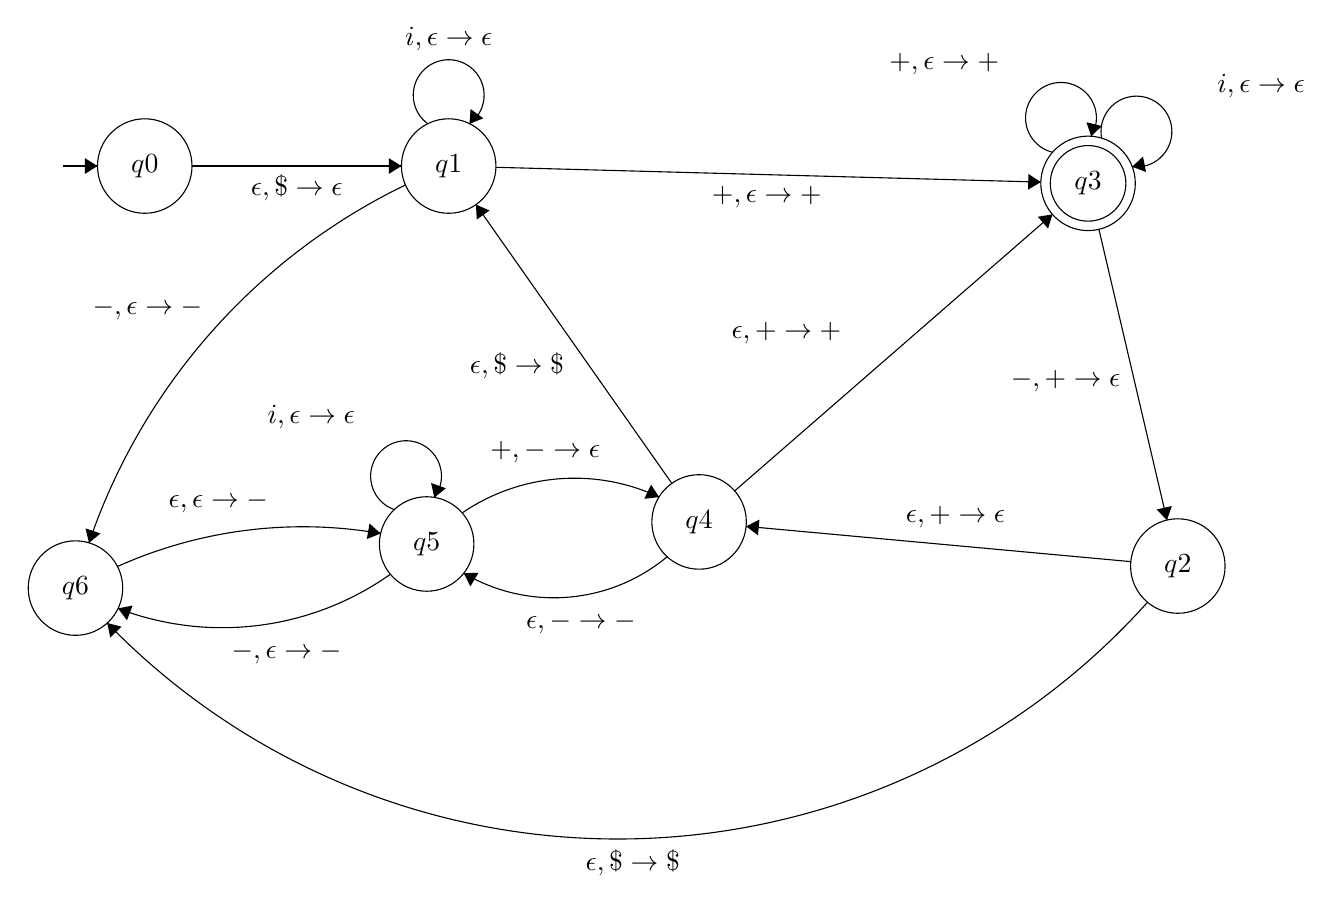
\begin{tikzpicture}[scale=0.2]
\tikzstyle{every node}+=[inner sep=0pt]
\draw [black] (8.4,-10) circle (3);
\draw (8.4,-10) node {$q0$};
\draw [black] (27.7,-10) circle (3);
\draw (27.7,-10) node {$q1$};
\draw [black] (68.3,-11.1) circle (3);
\draw (68.3,-11.1) node {$q3$};
\draw [black] (68.3,-11.1) circle (2.4);
\draw [black] (4,-36.8) circle (3);
\draw (4,-36.8) node {$q6$};
\draw [black] (26.3,-34) circle (3);
\draw (26.3,-34) node {$q5$};
\draw [black] (43.6,-32.6) circle (3);
\draw (43.6,-32.6) node {$q4$};
\draw [black] (74,-35.4) circle (3);
\draw (74,-35.4) node {$q2$};
\draw [black] (3.2,-10) -- (5.4,-10);
\fill [black] (5.4,-10) -- (4.6,-9.5) -- (4.6,-10.5);
\draw [black] (11.4,-10) -- (24.7,-10);
\fill [black] (24.7,-10) -- (23.9,-9.5) -- (23.9,-10.5);
\draw (18.05,-10.5) node [below] {$\epsilon,\$\rightarrow\epsilon$};
\draw [black] (30.7,-10.08) -- (65.3,-11.02);
\fill [black] (65.3,-11.02) -- (64.51,-10.5) -- (64.49,-11.5);
\draw (47.9,-11.23) node [below] {$+,\epsilon\rightarrow+$};
\draw [black] (69.163,-8.239) arc (190.95423:-97.04577:2.25);
\draw (79.29,-5.68) node [above] {$i,\epsilon\rightarrow\epsilon$};
\fill [black] (71.1,-10.04) -- (71.98,-10.38) -- (71.79,-9.4);
\draw [black] (26.377,-7.32) arc (234:-54:2.25);
\draw (27.7,-2.75) node [above] {$i,\epsilon\rightarrow\epsilon$};
\fill [black] (29.02,-7.32) -- (29.9,-6.97) -- (29.09,-6.38);
\draw [black] (4.857,-33.926) arc (161.21193:115.81358:39.304);
\fill [black] (4.86,-33.93) -- (5.59,-33.33) -- (4.64,-33.01);
\draw (12.08,-19.09) node [left] {$-,\epsilon\rightarrow-$};
\draw [black] (6.667,-35.43) arc (114.19381:80.11946:28.739);
\fill [black] (23.38,-33.33) -- (22.67,-32.7) -- (22.5,-33.69);
\draw (13.07,-32.05) node [above] {$\epsilon,\epsilon\rightarrow-$};
\draw [black] (24,-35.922) arc (-54.75838:-110.92835:18.515);
\fill [black] (6.7,-38.09) -- (7.27,-38.85) -- (7.63,-37.91);
\draw (17.4,-40.24) node [below] {$-,\epsilon\rightarrow-$};
\draw [black] (68.99,-14.02) -- (73.31,-32.48);
\fill [black] (73.31,-32.48) -- (73.62,-31.59) -- (72.65,-31.81);
\draw (70.39,-23.66) node [left] {$-,+\rightarrow\epsilon$};
\draw [black] (72.074,-37.7) arc (-41.84814:-135.86033:45.166);
\fill [black] (6.02,-39.02) -- (6.21,-39.94) -- (6.93,-39.25);
\draw (39.39,-53.36) node [below] {$\epsilon,\$\rightarrow\$$};
\draw [black] (71.01,-35.12) -- (46.59,-32.88);
\fill [black] (46.59,-32.88) -- (47.34,-33.45) -- (47.43,-32.45);
\draw (59.88,-32.99) node [above] {$\epsilon,+\rightarrow\epsilon$};
\draw [black] (28.553,-32.03) arc (124.37291:64.88023:12.644);
\fill [black] (41.06,-31.02) -- (40.55,-30.23) -- (40.12,-31.13);
\draw (33.83,-28.9) node [above] {$+,-\rightarrow\epsilon$};
\draw [black] (41.578,-34.805) arc (-50.16196:-120.5849:11.248);
\fill [black] (28.65,-35.85) -- (29.08,-36.69) -- (29.59,-35.83);
\draw (36.09,-38.33) node [below] {$\epsilon,-\rightarrow-$};
\draw [black] (45.86,-30.63) -- (66.04,-13.07);
\fill [black] (66.04,-13.07) -- (65.11,-13.22) -- (65.76,-13.97);
\draw (49.14,-21.36) node [above] {$\epsilon,+\rightarrow+$};
\draw [black] (41.87,-30.15) -- (29.43,-12.45);
\fill [black] (29.43,-12.45) -- (29.48,-13.4) -- (30.3,-12.82);
\draw (35.06,-22.67) node [left] {$\epsilon,\$\rightarrow\$$};
\draw [black] (24.256,-31.82) arc (250.89939:-37.10061:2.25);
\draw (18.97,-26.74) node [above] {$i,\epsilon\rightarrow\epsilon$};
\fill [black] (26.79,-31.05) -- (27.52,-30.46) -- (26.58,-30.13);
\draw [black] (66.054,-9.129) arc (256.46211:-31.53789:2.25);
\draw (59.17,-4.26) node [above] {$+,\epsilon\rightarrow+$};
\fill [black] (68.5,-8.12) -- (69.17,-7.46) -- (68.2,-7.22);
\end{tikzpicture}
\end{center}

\section{Definició formal de \pda{}}

\pda{} = \{ Q, $\Sigma$*, $\Gamma$*, $\delta$, q0, q3 \}

\begin{itemize}
\item Q = {q0, q1, q2, q3, q4, q5, q6}
\item $\Sigma$* = \{ +, -, \Return, $\epsilon$\}
\item $\Gamma$* = \{ +, - , \$, $\epsilon$\}
\item $\delta$ = Q X $\Sigma$* X $\Gamma$* $\rightarrow$ Q
\item q0 $\in$ Q
\item q6 $\subseteq{}$ Q
\end{itemize}

\subsection{Taula $\delta$ \pda{}}

\begin{table}[ht]
\caption{\label{tab:table-name} $\delta$ table for + and - inputs}
\centering
\begin{tabular}{ccccccccc}
\hline
\hline
input            & \multicolumn{4}{c}{+}            & \multicolumn{4}{c}{-}            \\
stack            & + & -          & \$ & $\epsilon$          & +          & - & \$ & $\epsilon$          \\
-\textgreater Q0 &   &            &    &            &            &   &    &            \\
Q1               &   &            &    & \{(Q3,+)\} &            &   &    & \{(Q6,-)\} \\
Q2               &   &            &    &            &            &   &    &            \\
Q3               &   &            &    & \{(Q3,+)\} & \{(Q2,$\epsilon$)\} &   &    &            \\
Q4               &   &            &    &            &            &   &    &            \\
Q5               &   & \{(Q4,$\epsilon$)\} &    &            &            &   &    & \{(Q6,-)\} \\
Q6               &   &            &    &            &            &   &    &     \\ \hline
\end{tabular}
\end{table}

\begin{table}[ht]
\caption{\label{tab:table-name} $\delta$ table for $\epsilon$ and \$ inputs}
\centering
\begin{tabular}{cccccccccc}
\hline
\hline
input            & \multicolumn{4}{c}{$\epsilon$} & \multicolumn{4}{c}{\$}                             \\
stack            & +   & -   & \$   & $\epsilon$           & +          & -          & \$          & $\epsilon$          \\
-\textgreater Q0 &     &     &      &             &            &            &             & \{Q1,\$)\} \\
Q1               &     &     &      & \{(Q1,$\epsilon$)\}  &            &            &             &            \\
Q2               &     &     &      &             & \{(Q4,$\epsilon$)\} &            & \{(Q6,\$)\} &            \\
Q3               &     &     &      & \{(Q3,$\epsilon$)\}  &            &            &             &            \\
Q4               &     &     &      &             & \{(Q3,+)\} & \{(Q5,-)\} & \{(Q1,\$)\} &            \\
Q5               &     &     &      & \{(Q5,$\epsilon$)\}  &            &            &             &            \\
Q6               &     &     &      &             &            &            &             & \{(Q5,-)\} \\ \hline

\end{tabular}
\end{table}


\section{Equivalència entre PDA i CFG}

Els PDA i el CFG són equivalents a nivell de potència.

Com diu al \textit{Theorem 2.20 de la referència [1]}, un llenguatge és lliure de context si i només si un autòmat de Pila és capaç de reconèixe’l i ho demostra al \textit{Lema 2.21 i al 2.27 [1]}.

Afirmem doncs, que podent representar l’autòmat \pda{} com un Push-Down autòmat existeix una $CFG$ capaç de generar tots els mots de \pda{}.

\section{Gramàtica lliure de context}

\textit{Veure Formal Definition de CFG, Definition 2.2, pàg 104 [1]}.

Denotem la construcció dels possibles mots com l'obligació d’afegir sempre un símbol + a un \wpda{} que tingui com a mínim el doble de símbols '+' que de '-'.

Expressem \pdaCFG{} = (V,T,P,S)

\begin{itemize}
\item V  = {S , A , B}
\item T = {+, -, i }
\item P = {
		S $\rightarrow$ A,
		A $\rightarrow$ B+A | B+B,
		B $\rightarrow$ -B+B+ | +B-B+ | +B+B- | BiB | $\epsilon$
      }
\end{itemize}

Aquesta gramàtica és capaç de generar tots els mots del L(\pda{}).

\section{Ambigüitat}

Una gramàtica lliure de context pot donar pas a diferents generacions d’un mateix mot, \textit{Definition 2.7, pàg 108 [1]}.

Podem detectar ambigüitat amb el mot \wpda on \wpda = '++-+', ens ajudem de \textit{l'eina sobre autòmats de la pàgina web d'Standford [8]} per demostrar-la.

Representem l'ambigüitat mitjançant les següents taules :

\begin{table}[ht]
\caption{\label{tab:table-name} Ambigüitat Figura 1}
\centering
\begin{tabular}{lll}
\hline
\hline
RULE                       & APPLICATION                        & RESULT \\
Start $\rightarrow$ S      & Start                              & S      \\
S $\rightarrow$ A          & \color{Blue}{S} & \color{Blue}{A}      \\
A $\rightarrow$ B+B        & \color{Blue}{A}                                  & \color{Blue}{B+B}    \\
B $\rightarrow$ $\epsilon$ & \color{Blue}{B}+B                                & +B     \\
B $\rightarrow$ +B-B+      & +\color{Blue}{B}                                 & +\color{Blue}{+B-B+} \\
B $\rightarrow$ $\epsilon$ & ++\color{Blue}{B}-B+                             & ++B-B+ \\
B $\rightarrow$ $\epsilon$ & ++-\color{Blue}{B}+                              & ++-+  \\ \hline
\end{tabular}
\end{table}

\begin{table}[ht]
\caption{\label{tab:table-name} Ambigüitat Figura 2}
\centering
\begin{tabular}{lll}
\hline
\hline
RULE                       & APPLICATION                        & RESULT  \\
Start $\rightarrow$ S      & Start                              & S       \\
S $\rightarrow$ A          & \color{Blue}{S} & \color{Blue}{A}       \\
A $\rightarrow$ B+B        & \color{Blue}{A}                                  & \color{Blue}{B+B}     \\
B $\rightarrow$ +B-B+      & \color{Blue}{B}+B                                & \color{Blue}{+B+B-}+B \\
B $\rightarrow$ $\epsilon$ & +\color{Blue}{B}+B-+B                            & ++B-+B  \\
B $\rightarrow$ $\epsilon$ & ++\color{Blue}{B}-+B+                            & ++-+B   \\
B $\rightarrow$ $\epsilon$ & ++-+\color{Blue}{B}                              & ++-+
\end{tabular}
\end{table}

\section{Chomsky Normal Form}

\textit{Veure Definició 2.8, pàg 109 [1]}.

\textit{“Qualsevol llenguatge lliure de context és generat per una gramàtica lliure de context en forma normal de Chomsky” - Theorem 2.9 - Michael Sipser}.

Per tant per generar la totalitat el L(\pda{}) ens n’assegurem passant la \pdaCFG{} a $CNF$. Emprem el programa \textit{JFLAP [6]} que segueix els passos descrits a \textit{Exemple 2.10, pàg 110 [1]}.

\begin{lstlisting}
S -> BF|EB|EA|BO|+|BE
B -> CB|i|BC|DL|DK|DJ|EI|EH|EG|EW|EV|EU|BT|DR|EQ|EP
F -> EA
E -> +
A -> EB|+|BE|EA|BO|BF
O -> EB
C -> i
D -> -
L -> EE
K -> EN
N -> BE
J -> BL
I -> DE
H -> DN
G -> BI
W -> ED
V -> EM
M -> BD
U -> BW
T -> CB
R -> BK
Q -> BH
P -> BV
\end{lstlisting}

\section{Referència al codi}

El codi del Push-Down Automata és a la classe PDA representada pels fitxers PDA.h i PDA.cpp a l'arrel del directori de la pràctica.

\section{Reconeixibilitat i Decidibilitat}

Tot llenguatge reconegut per un push-down autòmat determinista o indeterminista forma part dels llenguatges lliures de context i per definició \textbf{són reconeixibles per TM i decidibles}.

\section{Complexitat}

De la mateixa manera que amb un autòmat finit determinista, un autòmat push down determinista també contempla un nombre de passos similar a un dfa, en qualsevol cas el temps més gran que estarà processant tota l'entrada vindrà determinat per la llargada de \w{}. 

En aquest cas també hi ha la complexitat de treballar amb la pila, pot ser que apareguin nous estats i que la complexitat pugi, en qualsevol dels casos, en el nostre problema, ens mourem sempre dins de la Classe p. Llavors el nombre d'estats a atravessar vindrà donat per el n on n és la llargada de \w{} + el nombre de passos que farà amb la pila que com a molt en el nostre cas pot ser n també.

Per tant tinguent un temps O(n) * r on r és buidar la pila per complert, tindrem que com a molt r <= n i en el pitjor dels casos r = n. 

\begin{center}
O(n) * 2 = O(n) 
\end{center}

\textbf{I desestimant la constant 2 ens quedarà que la complexitat serà O(n) on  n = |\w{}|}.

\subsubsection{Dades extretes d'execucions}

Representem la taula següent amb execucions que contenen diferent nombre de files i columnes, s'hi ha afegit la columna n on es poden veure els tamanys de l'entrada. Per execucions inferiors de patrons de 40 files i 40 columnes el temps és despreciable. 

\begin{center}

\begin{table}[ht]
\caption{\label{tab:table-name} Data extraction}
\centering
\begin{tabular}{ccccc}
\hline
\hline
   & Cols & Rows & Clocks & N       \\ \hline
p4 & 40   & 40   & 0      & 1600    \\ \hline
p5 & 80   & 80   & 1      & 6400    \\ \hline
p6 & 160  & 160  & 2      & 25600   \\ \hline
p7 & 320  & 320  & 11     & 102400  \\ \hline
p8 & 640  & 640  & 41     & 409600  \\ \hline
p9 & 1280 & 1280 & 173    & 1638400 \\ \hline
\end{tabular}
\end{table}

\end{center}

\subsubsection{Representació gràfica de les execucions}

En aquest cas totes les execucions denoten un temps en clocks lineal en funció de l'entrada. Per tant determinem amb la gràfica la complexitat O(n) de l'autòmat PDA.

\begin{center}
\includegraphics[width=16cm]{copmlexpda}
\end{center}

\clearpage

\chapter{Turing Machine}

\section{Definició del Context}

Sigui \contextTM{} l'espai de funcionament lògic de la nostra màquina de Turing com l'espai estipulat a la \textit{Secció 3.Patrons[2]}. Per tant acabem d'adquirir totes les definicions assumides a l'enunciat del problema, veure \textit{[2]}.

\textbf{Fem les següents afirmacions sobre \preTM{} :}

\begin{itemize}
\item \w{} $\in$ $L^2$
\end{itemize}

\textbf{Fem les següents afirmacions sobre \postTM{} :}

\begin{itemize}
\item retorna -1 quan QReject
\item retorna t quan QAccept
\item loop altrament
\end{itemize}

on : $L^2$ definit a l'apartat \textit{4.Llenguatge Formal de l'enunciat del problema [2]}.

\section{Disseny descendent i pseudocodi}

Donat el problema presentat a l’\textit{exercici 5.3 que parla de Llenguatge Recursivament Enumerable, [2]}. Proposem el següent disseny descendent explicat també en pseudocodi per resoldre el problema PE on PE són els patrons explícits comentats a l'\textit{enunciat del problema [2] apartat 3.4}.

\begin{itemize}
\item Llegim patterns
\item return eval(patterns)
\end{itemize}

On patterns està compost dels patrons P1 i P2, i eval serà l'algoritme encarregat d'intentar decidir l'acceptació o rebuig de si P2 és un patró generacional fruit d'una evolució de P1 retornant el tick en el que P1 deriva a P2, \textbf{sempre que el pugui}.

Es pretén treballar amb patrons de manera genèrica, la millor manera de poder comparar si un patró és el mateix que un altre, és mitjançant la seva representació mínima. Per tant actuem sobre l’entrada per realitzar la següent operació sobre patrons:

\subsection{Minimització}

\begin{itemize}
\item PRE : Donat Py,x on x >= 0
\item POST : Retorna Py,0
\end{itemize}

Les minimitzacions contemplen la possibilitat que un patró estigui embolcallat dins de files amb cèl·lules inactives o columnes de cèl·lules inactives. \textit{Veiem apartat 3.1 Definició de patrons [2]}. La idea és extreure les files sobrants de cel·les inactives de la part superior i inferior del patró, transposar el patró, aplicar l'extracció de les cel·les inactives de la part superior i inferior altre cop i tornar a transposar el patró retornant així la seva representació mínima.

\begin{itemize}
\item Input P1
\item MinimizeByRows(P1)
\item Transpose(P1)
\item MinimizeByRows(P1)
\item Return Transpose(P1)

\end{itemize}

\subsection{Minimitzar per files}

La idea general és extreure les files plenes de cel·les inactives tant a principi com a final de patró. Comencem amb el patró inicial, només ens podem trobar cel·les inactives a les primeres files. Les regles són:

\begin{enumerate}
\item Ignorar les files que no continguin cel·les actives.
\item Quan trobem primera activa ho notifiquem i desem la fila en el patró resultant
\item per cada fila
	\begin{enumerate}
		\item Si no n’hi ha, acumulem fila en patró temporal
		\item si hi ha cel·la activa, persistim acumulat en patró resultant
	\end{enumerate}
\end{enumerate}

Per contra ignorarem al final totes les files acumulades que no tinguin cel·la activa.

\subsection{Transposició}

Operació matricial de transposició. \textit{Veiem Referència bibliogràfica [5].}

\subsection{Algoritme eval}

L’objectiu és anar contant el nombre de ticks que trigarà P1 a evolucionar a P2, per tant s’haurà de pensar l’evolució de P1 fent l’algoritme performTick que ens permeti crear el nou patró a partir de l’anterior.

A cada tick, el que fem és mirar cel·la a cel·la si P1 és igual en totes les posicions a P2. Per mirar això, fem un recorregut per les dues matrius alhora comparant les posicions entre elles.

\begin{itemize}
\item tickCounter = 0
\item While P1 != P2
	\begin{itemize}
	\item P1 = performTick(P1)
	\item tickCounter++;
	\end{itemize}
\item fi while
\item Return tickCounter
\end{itemize}

\subsection{Algoritme performTick}

Hem de preveure que el patró P1 pot créixer, per tant el patró resultant pot ser més gran que P1. Si afirmem que P1 creix en nombre de files i columnes cap a P1', podem dir que existeix un patró P1’ > P1 on :

\begin{center}
$P1' > P1 = (|files(P1’)|>|files(P1)|) ^ (|columnes(P1')>|columnes(P1)|)$
\end{center}

Per tant, si el patró P1 evoluciona fóra dels límits de P1, P1’ estarà preparat per poder representar-lo, en cas que no evolucioni fóra dels límits de la representació de P1, la minimització del mateix prèvia a la comparació farà la feina de representar-lo de manera inferior en nombre de files i columnes si escau.

Per cada cel·la de P1’ s’hi posa el resultat de la funció newCellValue que aplica les regles d’evolució per cada cel·la.

\subsection{Algoritme newCellValue}

Compararà donada una fila i una columna, les cel·les adjacents a aquesta fila i columna per determinar les caracterísitiques a seguir de l’evolució, explicades a \textit{l’apartat 3.4 Model, Enunciat de la pràctica [2]}.

Aquest algoritme fa un recorregut \textbf{constant} per les 8 posicions on hi pot haver un possible canvi. Concretament mira els veïns de la cel·la tractada i determina en funció de les normes especificades \textit{l’apartat 3.4 Model, Enunciat de la pràctica [2]} si la cel·la es manté en el seu estat o si rep un canvi.

\subsection{Referència al codi}

El codi de la Màquina de Turing es troba al directori / del directori de la pràctica, concretament en formen part :

\begin{itemize}
\item classe TM (TM.h i TM.cpp): Representa la màquina de Turing.
\item classe MatrixPattern (MatrixPattern.h i MatrixPattern.cpp): Representa la manera de tractar els patrons dins de la màquina de Turing.
\item classe Utils  (Utils.h i Utils.cpp): Eines útils per al tractament global de la mateixa màquina de Turing i pel main del programa.
\end{itemize}

\section{Reconeixibilitat del problema}

Definim \tmz{} com la primera versió de la \tmu{}, on la primera versió és la màquina Turing Reconeixible del llenguatge \ld{}.

\tm{} accepta tots els mots que pertanyen al llenguatge \ld{} descrit a l’\textit{apartat 5.3 Llenguatge Recursivament Enumerable, [2]}. Per construcció demostrem que el problema és Turing Reconeixible presentant un programa en C++.

Si un mot \w{} pertany a \ld{} llavors \tmz{} el reconeix, altrament loop.

En aquesta primera versió de la màquina \tmz{} ens centrem en la reconeixença del llenguatge i per tant només es contempla l’acceptació determinant que la màquina entrarà en un $QAccept$ quan es compleixi la igualtat en l’evolució. Altrament no podem determinar que la màquina (en aquesta primera versió) entri mai en un $QReject$.

\subsubsection{Exemple d'execució}

\textbf{Input : amb P1 i P2}

\begin{lstlisting}
++++++++++++
+----------+
+-++++++++-+
+-+------+-+
+-+-++++-+-+
+-+-++++-+-+
+-+-++++-+-+
+-+-++++-+-+
+-+------+-+
+-++++++++-+
+----------+
++++++++++++

------++++++------
------++++++------
------++++++------
------------------
------++++++------
-----++++++++-----
+++-++-++++-++-+++
+++-+++----+++-+++
+++-+++----+++-+++
+++-+++----+++-+++
+++-+++----+++-+++
+++-++-++++-++-+++
-----++++++++-----
------++++++------
------------------
------++++++------
------++++++------
------++++++------

\end{lstlisting}

\textbf{Output :}

\begin{lstlisting}
t = 3
\end{lstlisting}

\textbf{Concluïm que :}

P2 = P1$^3$


\section{Decidibilitat del problema}

La decidibilitat planteja el món dels problemes que presenten complexitats finites en la seva resolució. En aquest cas proposem diverses modificacions per \textbf{acostar} la implementació de \tm0{} -> \tm on \tm{} reconeix un conjunt més ampli de patrons.

En el nostre escenari el problema sabem que és reconeixible, però encara no podem afirmar que el problema sigui, o no, decidible, per tant anirem treballant sobre \tmz{} aplicant modificacions per intentar portar el problema al món dels decidibles. Per fer-ho estudiarem en les següents seccions els patrons i els seus comportaments.

\subsection{Comportaments de l’evolució de patrons}

Comentem les següents propietats detectades en el comportament de l’evolució de patrons.

\begin{itemize}
\item Derivació
\item Estabilització
	\begin{itemize}
	\item Extinció
	\end{itemize}
\item Oscil·lació
\item Creixement
\end{itemize}

\subsection{Derivació}

Per parlar de la decidibilitat del problema el primer cas que ens apareix és que el problema sigui turing reconeixible tal com s’ha demostrat a l’apartat [Reconeixibilitat del problema]. Llavors la derivació serà el que en decidibilitat es diu acceptació. Quan P1 evoluciona amb t = n a P2, llavors \w{} pertany al llenguatge L(\tm{}) i la màquina accepta.

\subsection{Estabilització}

\tmz{} no detecta quan $P2 != P1^t$, és a dir, no detecta cap cas en el qual es pugui afirmar que un patró P1 no tindrà una evolució a P2. L’estabilització d’un patró s’entén com :

\begin{center}
$P1^t = P1^{t+1}$
\end{center}

En aquest cas direm que el patró s’ha estabilitzat perquè :

\begin{center}
$\nexists P1^{t+n} != P1^t$
\end{center}

on : $n > 0$

I per tant en aquest cas es pot afirmar que P1 no evolucionarà mai fins P2 si no ho ha fet en $P1^t$.

Modifiquem \tmz{} -> \tmu{} perquè rebutgi ($QReject$) aquest cas. Amb aquesta acció podem descartar patrons com a candidats de formar part de \ld{}. S’ha acotat el conjunt de \w{} possibles a formar part de \ld{}.

\subsubsection{Exemple d'execució}

\textbf{Input : amb P1 i P2}

\begin{lstlisting}

++++++++++++
+----------+
+-++++++++-+
+-+------+-+
+-+-++++-+-+
+-+-++++-+-+
+-+-++++-+-+
+-+-++++-+-+
+-+------+-+
+-++++++++-+
+----------+
++++++++++++

------++++++------
------++++++------
------++++++------

\end{lstlisting}

\textbf{Output :}

t = -1

\textbf{Concluim que :}

$P2 != P1^8 \wedge P1^7 = P1^8$

\subsubsection{Extinció}

L’extinció d’un patró és un cas particular de l’estabilització. Un patró es pot extingir, i un cop extingit no pot tornar a aparèixer cap cel·la activa. Si $P1^y$ on y fa P1 extingit llavors :

\begin{center}
$\nexists P1^n \{n | n \in \mathbb{N} \wedge n > y\}$
\end{center}

\textbf{Veiem per la següent entrada :}

\begin{lstlisting}
----------
-+------+-
----------

-+-
-+-
\end{lstlisting}

\textbf{La següent sortida :}

t = -1


\textbf{conclusió}

P1 s'extingeix per t=1, P1$^2$ s'estabilitza.


\textbf{Veiem un altre exemple d’execució : }

\begin{lstlisting}
----------
-+------+-
----------

---
---
\end{lstlisting}

\textbf{La següent sortida}

t = 1

\textbf{Conclusió}

Fent l’anterior entrada estem detectant si P1 tendirà a la seva extinció.

\subsection{Oscil·lació}

El problema de l’oscil·lació comporta un repte més gran que els que ens hem plantejat fins ara, Detectem que un patró pot ser que oscil·li, és a dir que :

\begin{center}
$P1^1 = P1^3 = P1^5 = P1^n \{ n | n \in \mathbb{N} \% 2 \neq 0 \wedge n > 5 \} $
\end{center}

L’expressió anterior no està acotada a un finit de possibilitats. n és infinit. Per tant podria quedar oscil·lant amb la conseqüència que en termes de decidibilitat el problema entrés en loop. El repte de detectar aquest fet és plantejar-se la comparació en aquest cas amb una finestra de 3 patrons, i la comparació de $P1^{t+1}$ amb $P1^t$ i $P1^{t-1}$ on $t > 0$. D’aquesta manera, l'oscil·lació amb una finestra de 3 és decidible, presentem la màquina \tm{} com la màquina capaç de reconèixer aquestes oscil·lacions.

\textbf{Veiem per la següent entrada :}

\begin{lstlisting}
++++++++++++
+----------+
+-++++++++-+
+-+------+-+
+-+-++++-+-+
+-+-++++-+-+
+-+-++++-+-+
+-+------+-+
+-++++++++-+
+----------+
++++++++++++

++++++++++++
+----------+
+-++++++++-+
+-+------+-+
+-+-++++-+-+
+-+-+--+-+-+
+-+-++++-+-+
+-+------+-+
+-++++++++-+
+----------+
++++++++++++
\end{lstlisting}

\textbf{La següent sortida}

t = -1

\textbf{Conclusió}

El patró oscil·la amb finestra de 3 per t = 481.


El problema de l'oscil·lació és que en aquest cas ha entrat en joc una altra variable, la variable finestra. I és que si n és la finestra i n és infinit, llavors, totes les possibilitats en l'oscil·lació també ho són.

En aquest escenari n $\rightarrow \infty$, referenciant-nos al problema de l’aturada explicat a \textit{4.2. Halting problem, [1]}, veiem que requerim d'un problema indecidible per poder decidir la resposta del nostre problema. Necessitem saber abans de provar totes les possibilitats infinites de n si donat un mot \w{} la \tm{} no queda en loop, per poder afirmar que el problema representat amb la màquina \tm{} és decidible. \textbf{Aquest fet fa que el problema de detectar l'oscil·lació per n $\rightarrow \infty$,  sigui indecidible}.

\textbf{Veiem per la següent entrada :}

\begin{lstlisting}
-+-
-++
+-+

--+
---
\end{lstlisting}

\textbf{silence to the eternity...}

\textbf{Conclusió}

Si estudiem el cas de manera detallada, ens trobem que l'evolució d'aquest patró segueix la següent evolució:


$P1^0$
\begin{lstlisting}
-+-
-++
+-+
\end{lstlisting}

$P1^1$
\begin{lstlisting}
-++
+-+
--+
\end{lstlisting}

$P1^2$
\begin{lstlisting}
++-
-++
+--
\end{lstlisting}

$P1^3$
\begin{lstlisting}
+++
--+
-+-
\end{lstlisting}

$P1^4$
\begin{lstlisting}
-+-
-++
+-+
\end{lstlisting}


\subsection{Creixement}

El creixement és indeterminat, és a dir, detectar que un patró sempre creix és afirmar que per tots els $t > 0 P1^t < P1^{t+1} on t \rightarrow \infty$. Aquest cas no es pot determinar sense altre cop la màquina que reconeix el \textit{llenguatge del 4.2. Halting problem, [1]}. Per tant no podem determinar que un patró deriva a un altre en un t si tenim $\infty$ t per mirar, afirmant que l’evolució de P1 sempre creix.

\textbf{Si un patró sempre creix, podríem donar una resposta negativa (modificant \tm{}), el problema és determinar que sempre creix.}

\section{Complexitat respecte longitud d'entrada}

No podem afirmar que $L^2$ sigui decidible. Obligatòriament la màquina \tm{} haurà de parar per poder avaluar el temps.

Per tant el problema no pot ser avaluat en complexitat ja que no tenim la certesa que totes les execucions acabin. Com a requeriment, l’avaluació de complexitat especificada al \textit{capítol 7, primera frase del capítol [1]} ens estipula que sigui decidible.

De totes maneres, invertint hores a poder fer una avaluació de la complexitat sobre el nostre problema ens adonem que, amb les variables que tenim, podem limitar els valors d’aquestes variables perquè la màquina doni una resposta en un tick finit.

\subsection{Definició}

Definim $L^3$ com el llenguatge de la màquina \tml3{} capaç de reconèixer tots els mots $\in$ $L^2$ que miren si P1 evoluciona a P2 abans de $tf$ ticks. Sent $tf$ el valor màxim d’evolucions que se li permet fer a la màquina \tml3{} donat \w{} on:

\begin{center}
si \w{} $\in$ $L^3$ $\wedge$ \w{} $\in$ $L^2$ sent $L^3$ $\subset$ $L^2$
\end{center}

Amb \tml3{} ja no correm el risc d’entrar en un loop infinit, per tant ja no ens trobem amb oscil·lacions que no acaben mai, ni creixement cap a l’infinit. 

Per obtenir la complexitat total obtindrem la complexitat de cada una de les subtasques que realitza \tml3{} en funció de l’entrada.

\subsection{Complexitat desglosada \tml3{}}

La complexitat que estem estudiant deriva del desenvolupament del programa en C++. Per tant alguns algoritmes com la comparació que en el programa en C++ són O(n) si el portéssim a la definició formal de la TM(tenint en compte els moviments de la cinta) seria O(n2). Per tant la complexitat del nostre problema seria major.

\subsubsection{Input}

La primera tasca de \tml3{} és la de separar els 2 mots que formen \w{} en P1 i P2. Per tant la n que definirà la complexitat serà la llargada del mot \w{}. 

\begin{center}
n=|\w{}|
\end{center}

P1 i P2 se separen per un caràcter \Return que pot venir en qualsevol lloc del mot \w{}. Definim la posició on apareix aquest caràcter com a la variable u.

\begin{center}
p = |P1| = u-1


q = |P2| = n-u-1
\end{center}

En notació asimptotica la divisió dels mot \w{} en P1 i P2 seria O(n) :

\begin{center}
O(p) + O(q) = O(u-1) +  O(n - u - 1) = O(n)
\end{center}

Per comoditat es treballen P1 i P2 com a matrius, separant les files pel símbol \Return. D’aquesta manera tenim 2 variables més, x i y que representen el nombre de files i columnes que s’obtenen a partir de P1 i P2.

\begin{center}
x1 * y1 = p (per el mot P1)

x2 * y2 = q (per el mot P2)
\end{center}

Queda reflectit doncs que el fet de treballar amb una matriu no ens afecta en la complexitat, ja que la nostra n (p i q en el cas dels mots P1 i P2) és tot el mot. No ens hem de preocupar que el recorregut de la matriu sigui O(x*y) perquè al final recórrer tots els elements d’aquestes matrius acaben sent O(p) o O(q) per tant O(n).

\subsubsection{Primera Minimització}

Es minimitzen les dues parts de \w{}, P1 i P2. La minimització consta de 2 minimitzacions de fila i 2 traspocions. En el cas de la minimització per files es passa 1 sol cop per cada element de \w{}. Llavors tindrem:

\begin{center}
m(n) = O(n)  on m(n) és la funció de minimitzar per fila
\end{center}

En el cas de la transposició de les matrius, en funció de \w{} i no de x i y, es mira 1 sol cop cada element per tant:

\begin{center}
t(n) = O(n) on t(n) és la funció de transposició
\end{center}

Per un mot W’ la complexitat de la minimització seria:

\begin{center}
2*m(n) + 2*t(n) = 2*O(n) + 2*O(n) = 4*O(n) = O(n)
\end{center}

Com aquesta acció la fem tant per P1 com per P2 obtindríem una complexitat de 2*O(n) que acabarà sent O(n).

\subsubsection{Evolució del mot P1}

El mot P2 ja no es tornarà a modificar i només es farà servir per comparar a cada tick  amb  P1. 

Per tant observarem ara la complexitat d’aplicar les regles d’evolució per al mot P1. S’ha de tenir en compte que a partir de l’evolució la llargada de P1, és a dir p, pot variar, ja que el mot pot augmentar o disminuir. Això farà que p passi a ser una p’ en les diferents evolucions, de manera que s'haurà de mirar més o menys elements segons p'. Aquest fet però no ens afecta en termes de complexitat, ja que seguirem en O(p') o cosa que és el mateix O(n).

Per l’evolució del mot P1 passarem 1 sol cop per a cada caràcter i mirarem les 8 cel·les adjacents. Definim la funció d’evolució d’una cel·la com a ncv(x). Per tant:

\begin{center}
ncv(x) = 8*O(1)
\end{center}

Aplicat ncv(x) al mot P1 que ha de recórrer 1 cop tots els elements de P1 definint la funció ev(P1):

\begin{center}
ev(P1) = O(p)*ncv(x) = O(p)*8*O(1) =8*O(p) = O(n)
\end{center}

Un cop aplicada la funció d’evolució es torna a minimitzar el mot P1’ resultant. Definim la funció tick(P1) com a l'evolució de P1 + la minimització del mot P1' resultant.

\begin{center}
tick(P1) = ev(P1) + 2*m(p) + 2*t(p)
\end{center}

En termes de complexitat tick(n) serà:

\begin{center}
tick(P1) = O(p) + 2*O(p) + 2*O(p) = 5*O(p) = O(n)
\end{center}

\subsubsection{Generacions de T}

Per cada t s'haurà de comparar que els mots P1 i P2, en forma mínima, siguin iguals. Si no ho són es realitzarà una nova evolució sobre P1.

Per fer la comparació haurem de passar per cada element de P1 i P2 un sol cop i mirar que siguin iguals. Definim la funció de comparació com a eq(P1,P2). En termes de complexitat serà:

\begin{center}
eq(P1,P2) = \{ O(p) on p = | P1 | $\wedge$ | P1 | >= | P2 | \} = \textbf{O(n)}
\end{center}

Si tenim en compte MSPTM, és la modificació que mira si P1 s’estabilitza o oscil·la amb finestra f=3 haurem de fer 3 comparacions. Una per comparar P1 i P2, una altra per comparar P1 amb P1 de t-1 i una última per comparar P1 amb P1 de t-2 per tant:

\begin{center}
3* eq(P1,Px) = 3*O(n) = O(n)
\end{center}

Tenim doncs que la complexitat per a realitzar 1 tick, comptant la part de divisió de \w{} en P1 i P2 serà:

\begin{center}
O(p) + O(q) + 2*m(p) + 2*t(p) + 2*m(q) + 2*t(q) + G(P1,P2)

G(P1, P2)=  eq(P1,P2) + eq(P1, P1 t-1) + eq(P1, P1 t-2) + tick(P1)
\end{center}

Per a cada tick haurem de sumar un G(P1,P2) fins que MSPTM s’aturi per tant haurem de fer T vegades G(P1,P2). En termes de complexitat:

\begin{center}
T*G(P1,P2)= T* [ eq(P1,P2) + eq(P1, P1 t-1) + eq(P1, P1 t-2) + tick(P1) ] =  T * [ 3*O(n) + O(n) ] = T*O(n)
\end{center}

\section{Generació de patrons “God Mode”}

\tml3{} conté un mode d’execució anomenat "God Mode" executable amb el paràmetre "-d", veiem exemple d’execució: 

\begin{lstlisting}
./fc_4 -d
\end{lstlisting}


Ens apareix un menú com el següent (en l'execució queda ben indentat) :

\begin{lstlisting}
*********** You are in god mode ***********
*******************************************
*  Please enter one of following numbers  *
*                                         *
* Pattern Generation -----------------> 1 *
* Pattern from file  -----------------> 2 *
* Pattern from file show all matrix --> 3 *
* Pattern L3 from file ------------ --> 4 *
* Exit  ------------------------------> 0 *
*******************************************
\end{lstlisting}


Aquest és un programa de testeig i generació de patrons per poder estressar la complexitat del problema i poder crear diferents execucions mitjançant un tf finit. Els mots que genera contenen 2 patrons sempre de la mateixa dimensió amb els valors de cel·les actives i inactives escampades de manera aleatòria, en funció d’un \% d’aparicions, de cel·les actives, configurable.

Les sortides de la generació, opció 1 del menú mostrat anteriorment, escriuen un fitxer ".csv" que conté les dades relatives a n (files i columnes), el nombre de clocks que ha trigat la màquina, el nombre de ticks, el \w{} desglossat en P1 i P2 i informació sobre la configuració que ha utilitzat per a fer les execucions.

\textit{"Feel free to improve!"}

\subsubsection{Utilitzem "God Mode" per poder fixar $tf$. }

La idea és demostrar amb execucions que el problema té una complexitat lineal tal com s’explica a l’apartat Generacions de T.

Es genera l’execució amb els següents paràmetres sobre el "God Mode": 

\begin{lstlisting}
*********** You are in god mode ***********
*******************************************
*  Please enter one of following numbers  *
*                                         *
* Pattern Generation -----------------> 1 *
* Pattern from file  -----------------> 2 *
* Pattern from file show all matrix --> 3 *
* Pattern L3 from file ------------ --> 4 *
* Exit  ------------------------------> 0 *
*******************************************
> 1
* Please enter the following paramters : 
* How much patterns will be generated?> 50
* + symbol percentage of apparitions (0 -100) :> 30
* Number of rows :> 10
* Number of columns :> 10
* Growing factor :> 1.1
* statistics file name printed in csv?> logs/last.csv
* Print all matrix (true = 1, false = 0)? :>0
* Is L3 word? if not -1, else put a tick limit :> 60 
\end{lstlisting}

S’especifica :

\begin{itemize}
\item 50 patrons i 50 execucions de \tml3{}
\item El \% d’aparicions de cel·les actives a la matriu és de 30\%
\item Comencem amb una matriu de 10 files i 10 columnes
\item El creixement de les matrius serà multiplicar les files i les columnes per 1.1
\item Els resultats es desen a logs/last.csv
\item No mostra totes les matrius per pantalla
\item Per dir que el mot pertany a $L^3$ limitem els ticks a 60.
\end{itemize}

Es pot veure el fitxer original de l’execució al directori /logs/last.csv inclòs a l’entrega del problema.

\subsubsection{Dades extretes de l'execució}

De l'execució anterior s'ha extret un csv que mostra la taula següent : 

\begin{center}

\begin{table}[ht]
\caption{\label{tab:table-name} Data extraction}
\centering
\begin{tabular}{ccccc}
\hline
\hline
Rows & Columns & Clocks    & Ticks & n       \\ \hline
10   & 10      & 34719     & 100   & 100     \\ \hline
11   & 11      & 733       & 9     & 121     \\ \hline
13   & 13      & 27282     & 100   & 169     \\ \hline
15   & 15      & 25161     & 100   & 225     \\ \hline
17   & 17      & 62696     & 100   & 289     \\ \hline
19   & 19      & 59056     & 100   & 361     \\ \hline
21   & 21      & 62607     & 100   & 441     \\ \hline
24   & 24      & 66811     & 100   & 576     \\ \hline
27   & 27      & 77309     & 100   & 729     \\ \hline
30   & 30      & 86647     & 100   & 900     \\ \hline
33   & 33      & 103797    & 100   & 1089    \\ \hline
37   & 37      & 94671     & 100   & 1369    \\ \hline
41   & 41      & 155085    & 100   & 1681    \\ \hline
46   & 46      & 175812    & 100   & 2116    \\ \hline
51   & 51      & 209295    & 100   & 2601    \\ \hline
57   & 57      & 277091    & 100   & 3249    \\ \hline
63   & 63      & 307898    & 100   & 3969    \\ \hline
70   & 70      & 309872    & 100   & 4900    \\ \hline
77   & 77      & 429402    & 100   & 5929    \\ \hline
85   & 85      & 490101    & 100   & 7225    \\ \hline
94   & 94      & 541201    & 100   & 8836    \\ \hline
104  & 104     & 658871    & 100   & 10816   \\ \hline
115  & 115     & 869788    & 100   & 13225   \\ \hline
127  & 127     & 980636    & 100   & 16129   \\ \hline
\end{tabular}
\end{table}

\end{center}

\begin{center}

\begin{table}[ht]
\caption{\label{tab:table-name} Data extraction}
\centering
\begin{tabular}{ccccc}
\hline
\hline
Rows & Columns & Clocks    & Ticks & n       \\ \hline
140  & 140     & 1167342   & 100   & 19600   \\ \hline
154  & 154     & 1329948   & 100   & 23716   \\ \hline
170  & 170     & 1672998   & 100   & 28900   \\ \hline
188  & 188     & 1874516   & 100   & 35344   \\ \hline
207  & 207     & 2173532   & 100   & 42849   \\ \hline
228  & 228     & 2666196   & 100   & 51984   \\ \hline
251  & 251     & 3227996   & 100   & 63001   \\ \hline
277  & 277     & 3776230   & 100   & 76729   \\ \hline
305  & 305     & 4535434   & 100   & 93025   \\ \hline
336  & 336     & 5673440   & 100   & 112896  \\ \hline
370  & 370     & 6465573   & 100   & 136900  \\ \hline
408  & 408     & 7776788   & 100   & 166464  \\ \hline
449  & 449     & 9476329   & 100   & 201601  \\ \hline
494  & 494     & 11287831  & 100   & 244036  \\ \hline
544  & 544     & 13481008  & 100   & 295936  \\ \hline
599  & 599     & 16380963  & 100   & 358801  \\ \hline
659  & 659     & 19893390  & 100   & 434281  \\ \hline
725  & 725     & 23513986  & 100   & 525625  \\ \hline
798  & 798     & 28442093  & 100   & 636804  \\ \hline
878  & 878     & 34203490  & 100   & 770884  \\ \hline
966  & 966     & 41345181  & 100   & 933156  \\ \hline
1063 & 1063    & 50071367  & 100   & 1129969 \\ \hline
1170 & 1170    & 60121835  & 100   & 1368900 \\ \hline
1287 & 1287    & 72147782  & 100   & 1656369 \\ \hline
1416 & 1416    & 88056465  & 100   & 2005056 \\ \hline
1558 & 1558    & 105824920 & 100   & 2427364 \\ \hline
1714 & 1714    & 127344606 & 100   & 2937796 \\ \hline
1886 & 1886    & 153392593 & 100   & 3556996 \\ \hline
2075 & 2075    & 186453546 & 100   & 4305625 \\ \hline
\end{tabular}
\end{table}

\end{center}

On en la taula 4.2 és la continuació de la taula 4.1 i ambdós s'hi ha afegit la columna n que significa la llargada del patró del mot p on resideix realment el condicionant.

\clearpage

\subsubsection{Representació gràfica de l'execució.}

El següent gràfic mostra els clocks que ha trigat la \tml3 per realitzar la lectura de cada una de les execucions donat un n on n realiment és la que anteriorment s'ha denominat p. (seria el P1 del mot).

\begin{center}
\includegraphics[width=16cm]{complextm}
\end{center}

En termes de complexitat veiem que el llenguatge $L^3$  és O(n). Per tant veiem que té una complexitat lineal compresa en una complexitat Polinòmica.

Com que el disseny de \tml3{} és determinista i la complexitat és polinòmica podem dir que $L^3$ $\in$ CLASSE P \textit{secció 7.2 de [1]}.


\clearpage

\chapter{Continguts de l'entrega}

\begin{itemize}
\item Codi
\item Exemples $L^2$
\item Sortides
\item Documentació
\end{itemize}

\section{Codi}

El codi del programa es troba al directori arrel repartit en fitxers .h i .cpp. Es disposa de 4 parts diferenciades.

\begin{itemize}
\item DFA : fitxers DFA.h/.cpp i Alphabet.h/.cpp
\item PDA : fitxers PDA.h/.cpp i Alphabet.h/.cpp
\item TM : fitxers TM.h/.cpp, MatrixPattern.h/.cpp
\item Programa principal : main.h/.cpp i Utils.h/.cpp (i tots els anteriors)
\end{itemize}

La classe DFA conté el codi per l'autòmat finit determinista, la classe PDA conté el codi per l'autòmat de pila i la classe TM i MatrixPattern són els encarregats de gestionar el programa en C que representa la Màquina de Turing.

La classe Main i la classe Utils són complementaris per poder generar la fusió i que tot encaixi sense problema. La classe Alphabet conté les enumeracions utilitzades pel PDA i el DFA.

\section{Exemples $L^2$}

El directori data conté exemples de $L^2$ que poden ser executats a la fusió, és a dir al programa principal anomenat main.

\section{Sortides}

Utilitzant el paràmetre -d es pot entrar en mode Déu. El mode Déu permet rebre fitxers que continguin \w{} de \ld{}, i en algun dels casos permet generar-los també. En cas que es vulguin generar, es pot escollir la sortida en format csv on s'hi representen, el nombre de files i columnes de P1 on P1 és el patró que es farà evolucionar, els clocks de la màquina que triga a realitzar l'acció i el nombre de ticks que ha durat l'execució.

Addicionalment es demana informació sobre la generació que també s'escriu a la sortida.

Totes les sortides generades per nosaltres es poden trobar dins del directori logs del directori de l'entrega.

\section{Documentació}

Els fitxers per generar la documentació en pdf estan dins del directori documentation. L'informe consta d'un sol fitxer en format pdf que conté totes les descripcions i les conclusions a les quals hem arribat situat al directori arrel de l'entrega.

\section{That's all Folks}



\begin{thebibliography}{9}
\bibitem{FC}
Fundamental of Computation - Michael Sipser

\bibitem{patterns}
\href{http://ima.udg.edu/~rigau/FC/FC_patterns.pdf}{Problema Patterns (i.e., Cerca de Patrons) - Jaume Rigau}

\bibitem{Hopcroft}
\href{http://ima.udg.edu/~rigau/FC/MFAP.pdf}{Lexical analisys - part 4}

\bibitem{Manual UTM}
\href{http://ima.udg.edu/~rigau/FC/utm_read_me.pdf}{Universal Turing Machine - Manual}

\bibitem{MatrixPattern Transposition Wikipedia}
\href{https://en.wikipedia.org/wiki/Transpose}{MatrixPattern Transposition Wikipedia}

\bibitem{jflap}
\href{http://www.jflap.org/}{JFlap Automaton software}

\bibitem{chomsky normal form translator}
\href{https://mpeveler.com/assets/content/projects/cfg2cnf.php}{Generador de formes normals de chomsky}

\bibitem{Standford Automata web tool}
\href{https://web.stanford.edu/class/archive/cs/cs103/cs103.1156/tools/cfg/}{eina web de la pàgina web d’standford}

\end{thebibliography}

\printindex
\end{document}
